\documentclass[dutch]{uhphyspaper} 
%%%%%%%%%%%%%%%%%%%%%%%%%%%%%%
%       START DOCUMENT       %
%%%%%%%%%%%%%%%%%%%%%%%%%%%%%%
\usepackage{lipsum} % For demo purposes, remove 
\usepackage{listings} % Provides \lstinline{} for demo, remove
\usepackage{subcaption}

% Titles
\title{Ontsluieren van kleine, centrale beelden in gravitationele lenzen}
\runningtitle{}
\keywords{gravitationele lenzing, astrofysica, computationele fysica, Bayesiaanse statistiek, Monte-Carlo Markov Chain}

% Course information
\bachyear{$\mathit{3^{e}}$}
\course{Bachelorproef}
\date{\today}

% Authors, supervisors, principle investigator (PI, promotor)
\author[1]{Yara Roelen}
\author[1$^{\dagger}$]{Jori Liesenborgs} % Promotor: Dagger here signifies that the PI is the main correspondent

% Author affiliations
\affil[1]{UHasselt, Agoralaan, 3590 Diepenbeek, België}
\affil[1]{Applied Computer Science Lab}
\affil[1$^{\dagger}$]{UHasselt, EDM, Agoralaan, 3590 Diepenbeek, België} % Dagger here signifies that the PI is the main correspondent

% PI contact info, do not remove
\pitel{+3211268429}
\pimail{jori.liesenborgs@uhasselt.be}

%%%%%%%%%%%%%%%%%%%%%%%%%%%%%%
%       START DOCUMENT       %
%%%%%%%%%%%%%%%%%%%%%%%%%%%%%%
\begin{document}
\maketitle\thispagestyle{fancy} 
% pagestyle ensures header is present

% Each section is placed in a separate file to better organise your text
% You can find these files in the Sections folder
\section*{ABSTRACT}
% Edit below
\textbf{Bij gravitationele lenzing kan het voorkomen dat een object afgebeeld wordt op meerdere beelden. Soms komt het voor dat een beeld achter de lens (een zware massa) staat. Dan kan nuttige informatie over de massaverdeling van de lens niet gevonden worden.\\ \\
Om toch informatie te kunnen bekomen over de zware massa moet het beeld dat achter de zware massa staat gevonden worden. Dat wordt gedaan op drie verschillende manieren, allen gebaseerd op de stelling van Bayes: de kansdichtheid, het Metropolis algoritme en de emcee library. Alle drie de methodes geven gelijkende resultaten. \\ \\
Eerst werd het Metropolis algoritme uitgetest. Dat werkt goed vanaf een voldoende groot aantal samples. Nadien werd met de kansdichtheid en het Metropolis algoritme informatie over een signaal met achtergrondruis verzameld. Ook dit werkte goed. Bij het signaal en de ruis waren er twee onbekende parameters. Dit werd uitgebreid naar zes parameters, de parameters van de zware massa (een sersic). Ook het afschatten van alle parameters van een sersic is gelukt. \\ \\
Het is ook gelukt om de parameters van een systeem bestaande uit twee sersics af te schatten. Er werd een zware massa op een werkelijke achtergrond (gemodelleerd door NASA) geplaatst. Hier werd er opnieuw geprobeerd om de parameters van de zware massa zo goed mogelijk af te schatten, zodat de achtergrond zichtbaar wordt. Dit is niet volledig gelukt, doordat de achtergrond te ruisig was en er op die manier geen nauwkeurige afschatting van de parameters van de sersic gemaakt konden worden. In de toekomst zou voor dit probleem AI gebruikt kunnen worden.}
\newline
\rule[1.5ex]{\linewidth}{0.4pt}

\section{INTRODUCTIE}
Gravitationele lenzing is een effect dat optreedt wanneer licht afgebogen wordt door het gravitatieveld van massieve objecten, zoals sterrenstelsels of clusters. Deze objecten bevatten doorgaans veel donkere materie. \cite{informationesoorg-no-date}. De afbuiging van het licht kan zowel Newtoniaans als relativistisch afgeleid worden. De Newtoniaanse afleiding voor een hyperbolische baan is te vinden in \cref{appendix: newton}. In tegenstelling tot klassieke lenzing, waarbij één object wordt afgebeeld op één ander object, kan bij gravitationele lenzing één object afgebeeld worden op meerdere objecten \cite{unknown-author-2022}. Dit is te zien in \cref{fig:grav lens}. 
\begin{figure}
    \centering
    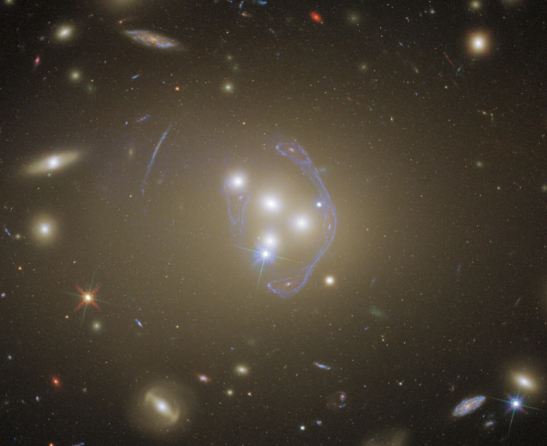
\includegraphics[width=0.95\linewidth]{Figures/gravitationele_lens.png}
    \caption{Gravitationele lens, foto van \cite{unknown-author-no-date-gravlens}}
    \label{fig:grav lens}
\end{figure}
Dit wordt bepaald door de lensvergelijking. De afleiding van de lensvergelijking in 1D is te vinden in \cref{appendix:lensvergelijking}.\\ \\
Om meer informatie te kunnen krijgen over de gravitationele lens kan het heel nuttig zijn om alle beelden die de lens genereert terug te vinden. De grotere beelden gaan voornamelijk informatie geven over de vorm van de lens, terwijl de kleinere beelden veelal informatie geven over de massaverdeling ervan. \\ \\
Soms kan het voorkomen dat een object afgebeeld wordt achter de zware massa zelf. Op \cref{fig:grav lens} zijn vijf beelden te zien. Het aantal beelden dat de lens genereert is berekend, en is gelijk aan negen. Dat wil zeggen dat er nog vier beelden zijn die niet gevonden worden doordat ze achter de lens zelf staan. Deze vier beelden geven echter wel cruciale informatie over de massaverdeling van de lens. Omdat het geweten is dat de zware massa voornamelijk uit donkere materie bestaat zou informatie over de massaverdeling ervan meer inzichten kunnen geven in donkere materie. Het doel van deze bachelorproef is het wegwerken van de zware massa op de voorgrond, om de achtergrond waar te kunnen nemen. \\ \\
Er bestaan al een heel aantal manieren waarop dit gedaan kan worden. Voorbeelden hiervan zijn IMFIT \cite{chen-2020}, \cite{erwin-2015} en GALFIT \cite{peng-2010}, \cite{unknown-author-no-date-galfit}.
In deze bachelorproef wordt er gebruik gemaakt van Bayesiaanse statistiek in de toekomst zou er ook met deep learning gewerkt kunnen worden.




\section{THEORIE}
\subsection{Bayesiaanse statistiek}
In onze opleiding wordt enkel kennisgemaakt met frequentistische statistiek. In deze vorm van statistiek wordt er steeds gekeken naar tellingen. Er wordt ook aangenomen dat er nog niets geweten is over het systeem. Er wordt aan de tellingen begonnen zonder voorgaande kennis. Als je wil weten wat de kans is dat je een vijf gooit met een zeszijdige dobbelsteen, dan gooi je 1000 keer met de dobbelsteen en tel je het aantal keer dat je een vijf gooide.\\ \\
In de Bayesiaanse statistiek wordt de kans geïnterpreteerd als de mate van kennis die vergaard is over het systeem.
In de Bayesiaanse statistiek wordt vaak aangenomen dat er al kennis is van het systeem. Er wordt begonnen met een prior kansverdeling, die modelleert wat er al gekend is van het systeem. Kans wordt gezien als een dynamisch gegeven dat continu verandert op basis van nieuwe beschikbare gegevens. Op basis van deze informatie wordt de kansdichtheidsfunctie continu aangepast. Zo kan er toegewerkt worden naar een posterior kansdichtheid die weergeeft wat er uiteindelijk geweten is over het systeem. Op basis van deze posterior kunnen er probabilistische uitspraken gedaan worden over het systeem. \cite{walker-2005}.\\ \\
In deze statistiek wordt er gewerkt met een belangrijke formule, de stelling van Bayes. Deze is terug te vinden in \cref{for:bayes} \cite{hayes-2024}.
\begin{equation}
    P(H|E)=\frac{P(E|H)\cdot P(H)}{P(E)}
    \label{for:bayes}
\end{equation}
De parameters van \cref{for:bayes} worden overlopen\cite{unknown-author-2023}.
\begin{itemize}
    \item $H$: de hypothese
    \item $E$: het bewijs, de waarneming
    \item $P(H|E)$: de posterior, dit is de kans op de hypothese gegeven het geobserveerde bewijs E. Dit is waar naar opzoek gegaan wordt.
    \item $P(E|H)$: de kans op het observeren van E, gegeven de hypothese. Dit wordt de likelihood genoemd. Dit toont aan hoe compatibel de gemeten data is met de hypothese. 
    \item $P(E)$: dit is de marginale waarschijnlijkheid. Deze is dezelfde voor alle hypotheses
    \item $P(H)$: de prior, dit is de schatting van de kans op een hypothese H, voordat er bewijs waargenomen is.
\end{itemize}
\subsection{Monte Carlo en het metropolis algoritme}
Monte Carlo is een reeks van computationele algoritmes die gebruikt kunnen worden om te samplen uit een kansdichtheid. De term Monte Carlo wijst op het feit dat er gebruik gemaakt wordt van willekeurige gebeurtenissen, dit gaat verder dan het sampelen uit een kansdichtheid, maar dat is voor deze bachelorproef niet relevant. Door veelvuldige herhaling van hetzelfde algoritme, maar met een andere beginpositie kan een kansdichtheid gegenereerd worden \cite{wikipedia-bijdragers-2023}\cite{kenton-2023}. Als er een helder sterrenstelsel staat voor het beeld dat nodig is voor een volledige waarneming van de gravitationele lens, dan kan dat stelsel weggefilterd worden door de parameters van het stelsel, en de parameters van het beeld af te schatten. Als alle parameters gekend zijn, kan het beeld gereconstrueerd worden.\\ \\
In deze bachelorproef wordt er steeds een dataset gesimuleerd. Uit deze dataset worden samples genomen. Die samples worden geïnterpreteerd als de af te schatten parameters. Het nemen van samples wordt gedaan met behulp van Monte Carlo. Omdat er gewerkt wordt met kansverdelingen van meerdere dimensies wordt gebruik gemaakt van Markov-Chain Monte Carlo \cite{unknown-author-2023-MCMC}.\\ \\
Het algoritme dat in deze bachelorproef gebruikt werd, is het Metropolis–Hastings algoritme. Dit is gebaseerd op Markov-Chain Monte Carlo. Het algoritme werkt als volgt\cite{unknown-author-no-date}, \cite{thijssen-2007}:\\ \\
Zij f(x) een functie die evenredig is met de gewenste kansdichtheidsfunctie. Noem f(x) de target functie. Heel vaak komt deze target overeen met de posterior van de stelling van Bayes. Het algoritme gaat als volgt:
\begin{enumerate}
    \item initialisatie: kies een random punt $x_{t}$ als eerste observatie, of kies een punt op basis van eerder verkregen info van het systeem.
    \item herhaal voor elke iteratie t:
    \begin{itemize}
        \item Er wordt een nieuwe kandidaat x' voorgesteld, door bij de vorige waarde een waarde op te tellen die random gekozen wordt uit de normale verdeling met als gemiddelde 0 en als standaardafwijking 0.1 (er zou ook een andere kansverdeling gebruikt kunnen worden, ook de standaardafwijking is afhankelijk van de situatie).
        \item De acceptatieratio $\alpha$, $\alpha=\frac{f(x')}{f(x_{t})}$ wordt bepaald. Dit wordt gebruikt om te bepalen of de nieuwe waarde geaccepteerd wordt, of dat er verder gewerkt wordt met de oorspronkelijke waarde. 
        \item Er wordt bepaald of de waarde geaccepteerd of verworpen wordt. Er wordt een random getal $u$ tussen 0 en 1 gegenereerd. Als $u\leq\alpha$ dan wordt de toestand geaccepteerd. Als $u>\alpha$ dan wordt de kandidaat verworpen en wordt er verder gegaan met de oorspronkelijke waarde.
    \end{itemize}
\end{enumerate}
Naast dit algoritme wordt er ook gewerkt met de emcee library \cite{unknown-author-no-date-emcee}. Deze werkt ook op basis van Markov-Chain Monte Carlo, maar heeft als grote voordeel dat er op voorhand niks geweten moet zijn over de kansverdeling. In de emcee library wordt er gebruik gemaakt van een aantal walkers, die allemaal onafhankelijk van elkaar de kansverdeling gaan afstappen. Zij gaan zelf hun stapgrootte en dergelijke aanpassen aan de situatie. De walkers starten vanop verschillende beginposities en werken toe naar een target kansverdeling. 











 % May be removed if unnecessary

\section{RESULTATEN EN DISCUSSIE}
Het onderzoek werd gedaan met behulp van de programmeertaal Python (versie 3.12). Er werd gebruik gemaakt van de standaard library \cite{unknown-author-no-date-python}. Verder werden volgende library's nog gedownload:
\begin{itemize}
    \item numpy (versie 1.26.4)
    \item matplotlib.pyplot (versie 3.8.3)
    \item emcee (versie 3.1.4)
    \item scipy (versie 1.12.0)
\end{itemize}
\subsection{Visualisatie van het Metropolis algoritme}
In het Metropolis algoritme worden samples genomen van een gewenste kansdichtheid. Er wordt steeds begonnen vanaf een gekozen positie. In het begin kan er niet veel afgeweken worden van die positie doordat er steeds maar kleine stapjes gezet worden. De eerste data die gegenereerd wordt komt dan ook nog niet goed overeen met de gewenste kansverdeling. Daarom worden steeds de eerste gegenereerde datapunten weggegooid. \\ \\
Om dit te laten zien werd een klein programma geschreven dat probeert om een kansverdeling na te maken. Om de 90 stappen wordt de stand van zaken afgebeeld op een figuur waarop zowel de huidige kansverdeling als de gewilde kansverdeling te zien zijn. \\ \\Deze visualisatie is te zien in \cref{fig: visualisatie_metropolis}.
\begin{figure}
    \centering
    \begin{minipage}{0.49\linewidth}
        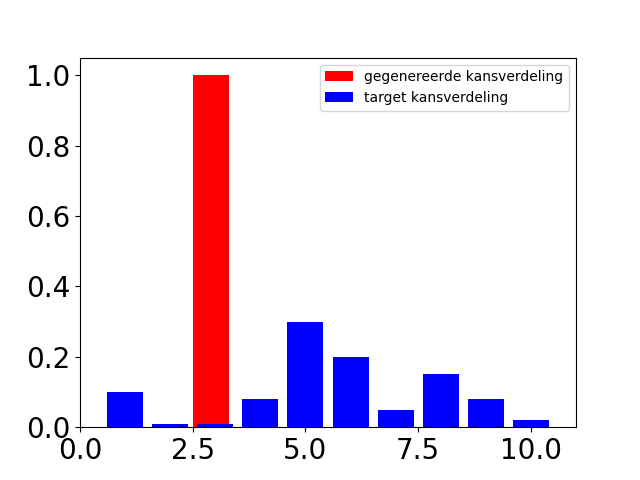
\includegraphics[width=\linewidth]{Figures/goede_visualisatie_3/visualisatie_1.png} 
        \subcaption{na stap 0}
    \end{minipage}
    \hfill
    \begin{minipage}{0.49\linewidth}
        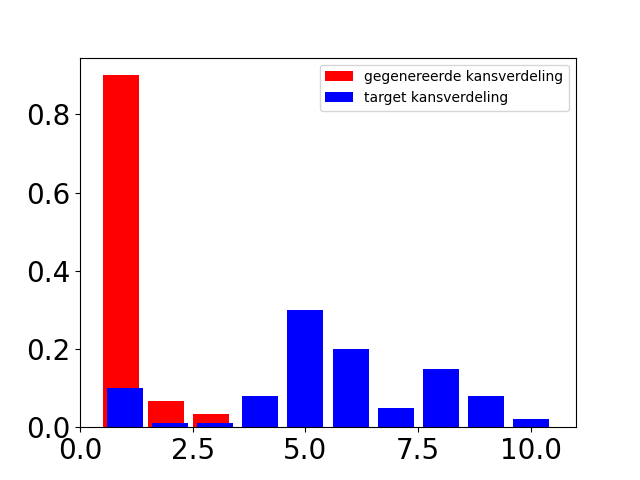
\includegraphics[width=\linewidth]{Figures/goede_visualisatie_3/visualisatie_90.png}
        \subcaption{na stap 90}
    \end{minipage}
    \begin{minipage}{0.49\linewidth}
        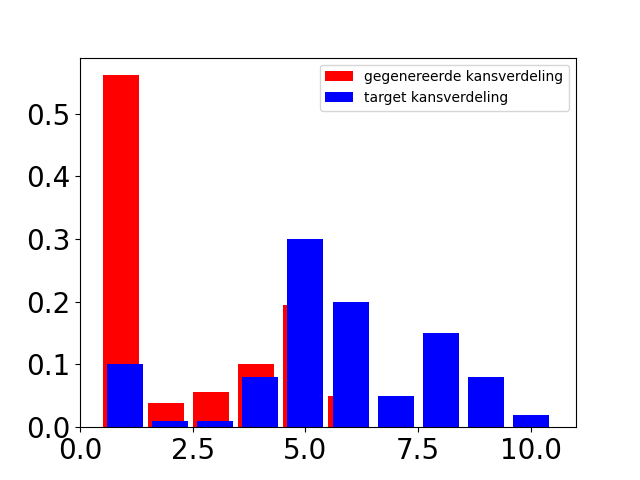
\includegraphics[width=\linewidth]{Figures/goede_visualisatie_3/visualisatie_180.png} 
        \subcaption{na stap 180}
    \end{minipage}
    \hfill
    \begin{minipage}{0.49\linewidth}
        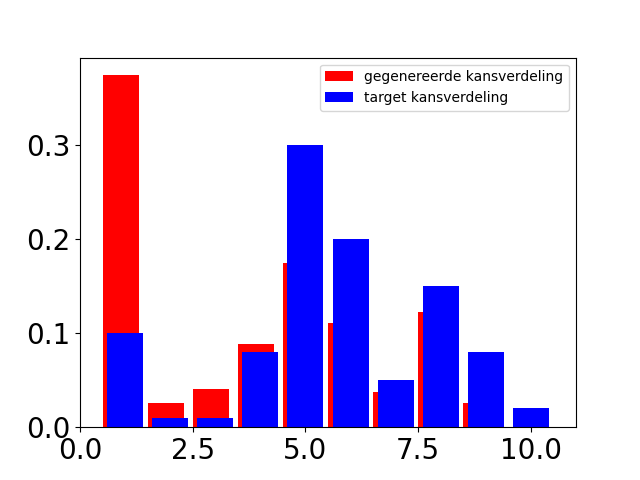
\includegraphics[width=\linewidth]{Figures/goede_visualisatie_3/visualisatie_270.png}
        \subcaption{na stap 270}
    \end{minipage}
    \begin{minipage}{0.49\linewidth}
        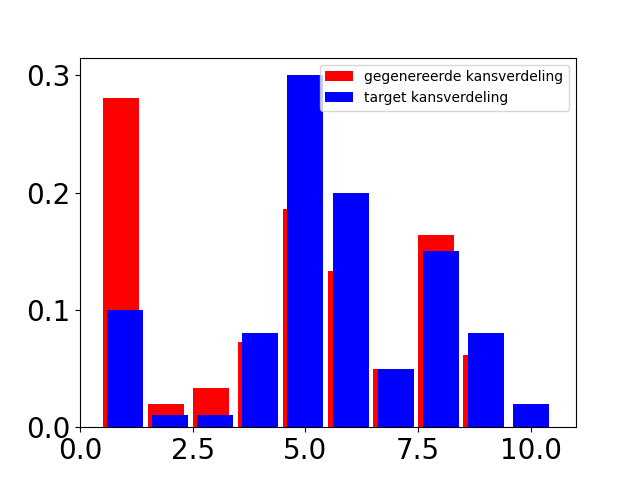
\includegraphics[width=\linewidth]{Figures/goede_visualisatie_3/visualisatie_360.png} 
        \subcaption{na stap 360}
    \end{minipage}
    \hfill
    \begin{minipage}{0.49\linewidth}
        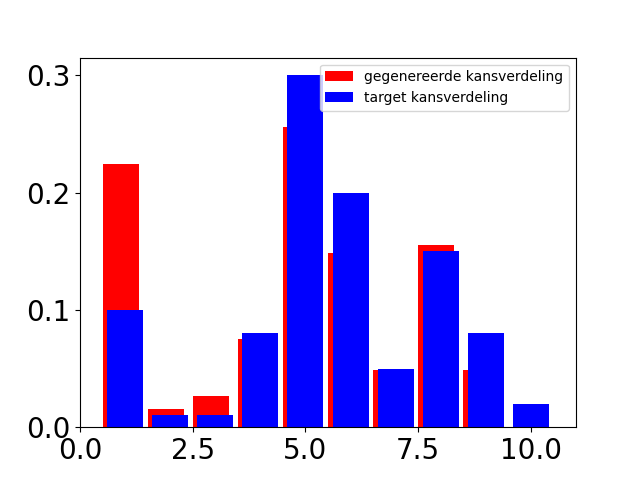
\includegraphics[width=\linewidth]{Figures/goede_visualisatie_3/visualisatie_450.png}
        \subcaption{na stap 450}
    \end{minipage}
    \begin{minipage}{0.49\linewidth}
        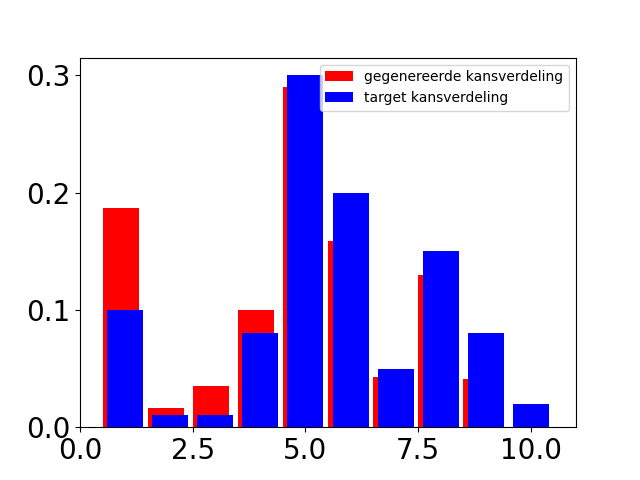
\includegraphics[width=\linewidth]{Figures/goede_visualisatie_3/visualisatie_540.png} 
        \subcaption{na stap 540}
    \end{minipage}
    \hfill
    \begin{minipage}{0.49\linewidth}
        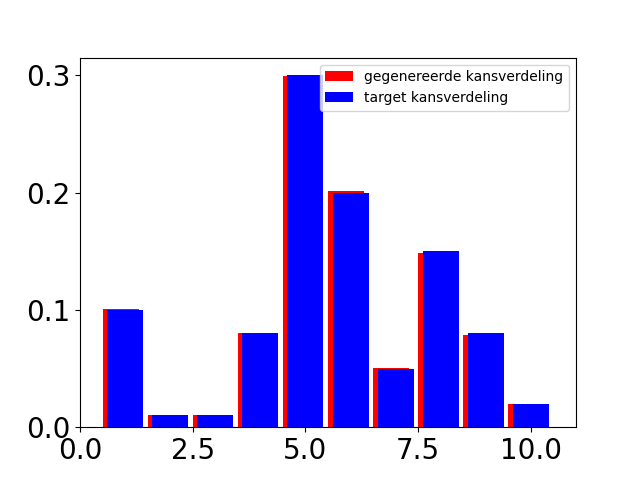
\includegraphics[width=\linewidth]{Figures/goede_visualisatie_3/visualisatie_1000000.png}
        \subcaption{na stap 100\_000}
    \end{minipage}
\caption{Visualisatie van het proces waarin toegewerkt wordt naar de gewenste kansverdeling. Op de bovenstaande figuren is de stand van zaken te zien na een vermeld aantal stappen. Het blauwe histogram is de target kansverdeling, het rode histogram is de huidige gesampelde kansverdeling.}
\label{fig: visualisatie_metropolis}
\end{figure}
Zoals te zien in de visualisatie (\cref{fig: visualisatie_metropolis}) heeft het algoritme wat tijd nodig om tot zijn target kansverdeling te komen. Na 90 stappen wordt de target kansverdeling nog niet benaderd, na 100\_000 stappen wordt bijna exact dezelfde kansverdeling als de target kansverdeling gevonden. Doordat die tijd nodig is om naar de target kansverdeling te gaan, heeft het pas zin om samples te halen uit de gewenste kansverdeling vanaf het moment dat de target benaderd wordt. Om die reden worden heel vaak de eerste samples weggegooid. Zo start de sampeling pas vanaf het moment dat de target kansverdeling bij benadering bereikt is. Het exacte punt waarop de kansverdeling goed genoeg benadert wordt, is niet gekend.
\subsection{Signaal en achtergrondruis: stelling van Bayes, het Metropolis algoritme en de emcee library}
Voor er gestart werd met het schatten van de parameters van het sterrenstelsel en het beeld dat erachter staat, werd er gestart met het afschatten van een amplitude van een signaal (A) in de aanwezigheid van achtergrondruis (B) \cite{sivia-2006}. Op de $x$-as staat de te meten variabele. De situatie is te zien in \cref{fig:AB}. 
\begin{figure}
    \centering
    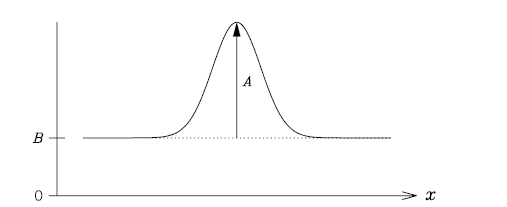
\includegraphics[width=0.95\linewidth]{Figures/Schermafbeelding 2024-05-13 144419.png}
    \caption{het meest eenvoudige geval van en signaal met amplitude A op een vlakke achtergrond van sterkte B. Foto uit \cite{sivia-2006}.}
    \label{fig:AB}
\end{figure}
Het is eenvoudig in te zien dat het aantal tellingen op een positie $x_{k}$ evenredig is met de sterkte van de achtergrond B plus het signaal A. Er wordt aangenomen dat de piek van het signaal Gaussisch is. Beschouw een piek met breedte $w$ gecentreerd rond $x_{0}$, dan is de waarde op positie $k$ gegeven door \cref{for:signaal}
\begin{equation}
D_{k}=n_{0}\left(Ae^{-\frac{(x_{k}-x_{0})^{2}}{2w^{2}}} + B\right)
\label{for:signaal}
\end{equation}
Hierin is $n_{0}$ een constante gerelateerd aan de duurtijd van de meting. \\ \\
Dit werd gedaan gebruikmakende van de stelling van Bayes. Eerst werd er gewerkt met de kansdichtheidsfunctie en later ook met het Metropolis algoritme en de emcee library. \\ \\Van de piek van het signaal en de achtergrond werd een 2D histogram gemaakt. De waarden werden ook gemarginaliseerd zodat ook het signaal en de achtergrond apart geplot konden worden. Ook werden op verschillende meetpunten $k$ het aantal tellingen bepaald. De figuren voor 1842 metingen en 25 databins, gebruikmakende van de kansdichtheid, het metropolis algoritme en de emcee library zijn te vinden in \cref{fig:AB-bay} en \cref{fig:AB-met-mc}. Merk op dat er steeds met dezelfde dataset gewerkt wordt in alle drie de voorbeelden.
\begin{figure}
    \begin{minipage}{0.95\linewidth}
        \centering
        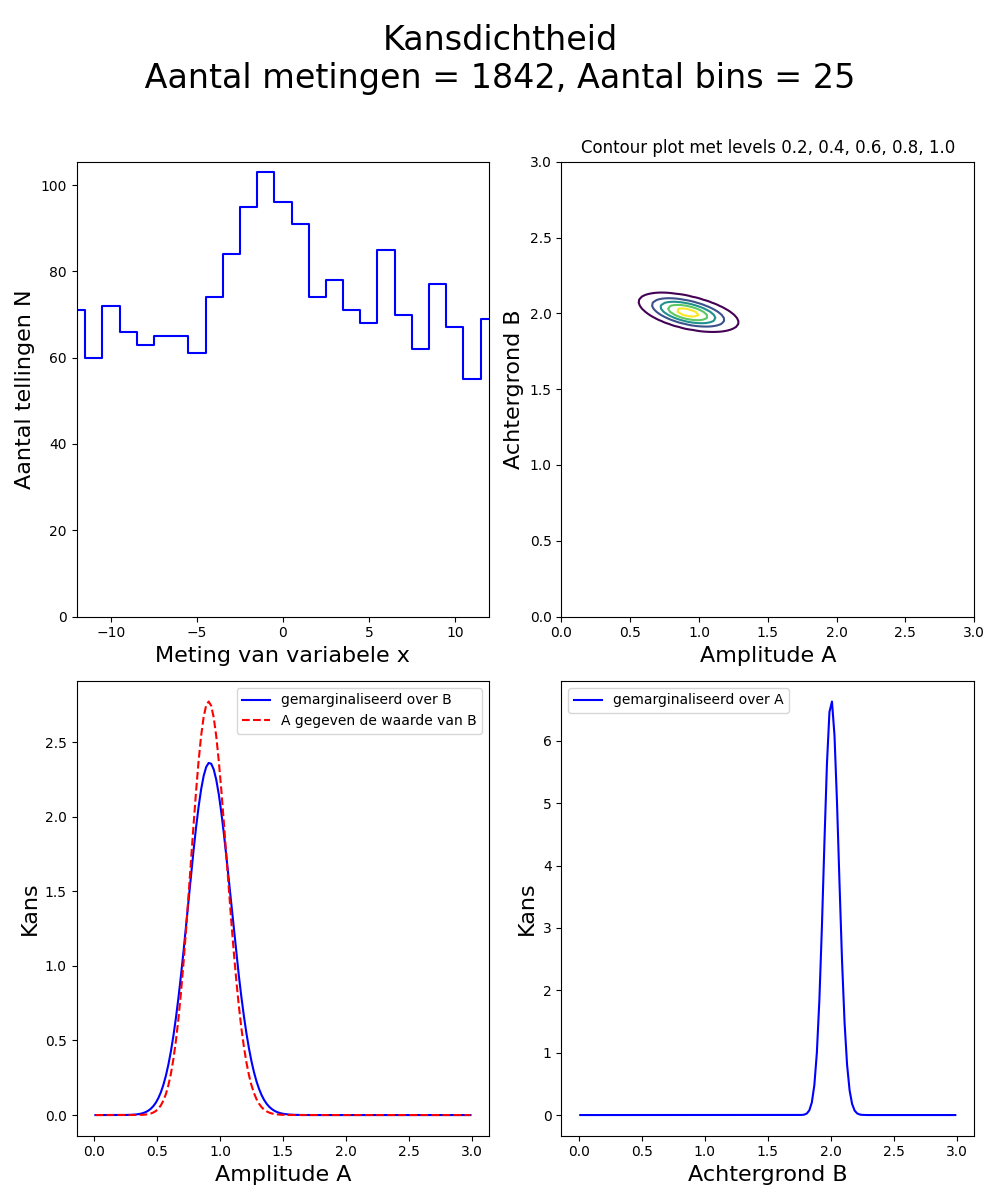
\includegraphics[width=0.95\textwidth]{Figures/figurenset1.png}
        \label{fig:AB-bayes}
    \end{minipage}
\caption{Het resultaat van het plotten van het signaal met ruis gebruikmakende van de kansdichtheid. Op de figuur linksboven staat steeds het aantal tellingen per datapunt, op de figuur rechtsboven staat het 2D histogram van het signaal met de achtergrond. Op de figuur linksonder staat de amplitude van het signaal, gemarginaliseerd over de achtergrond. Linksonder staat de achtergrond, gemarginaliseerd over het signaal.}
\label{fig:AB-bay}
\end{figure}
\begin{figure}
\begin{minipage}{0.98\linewidth}
        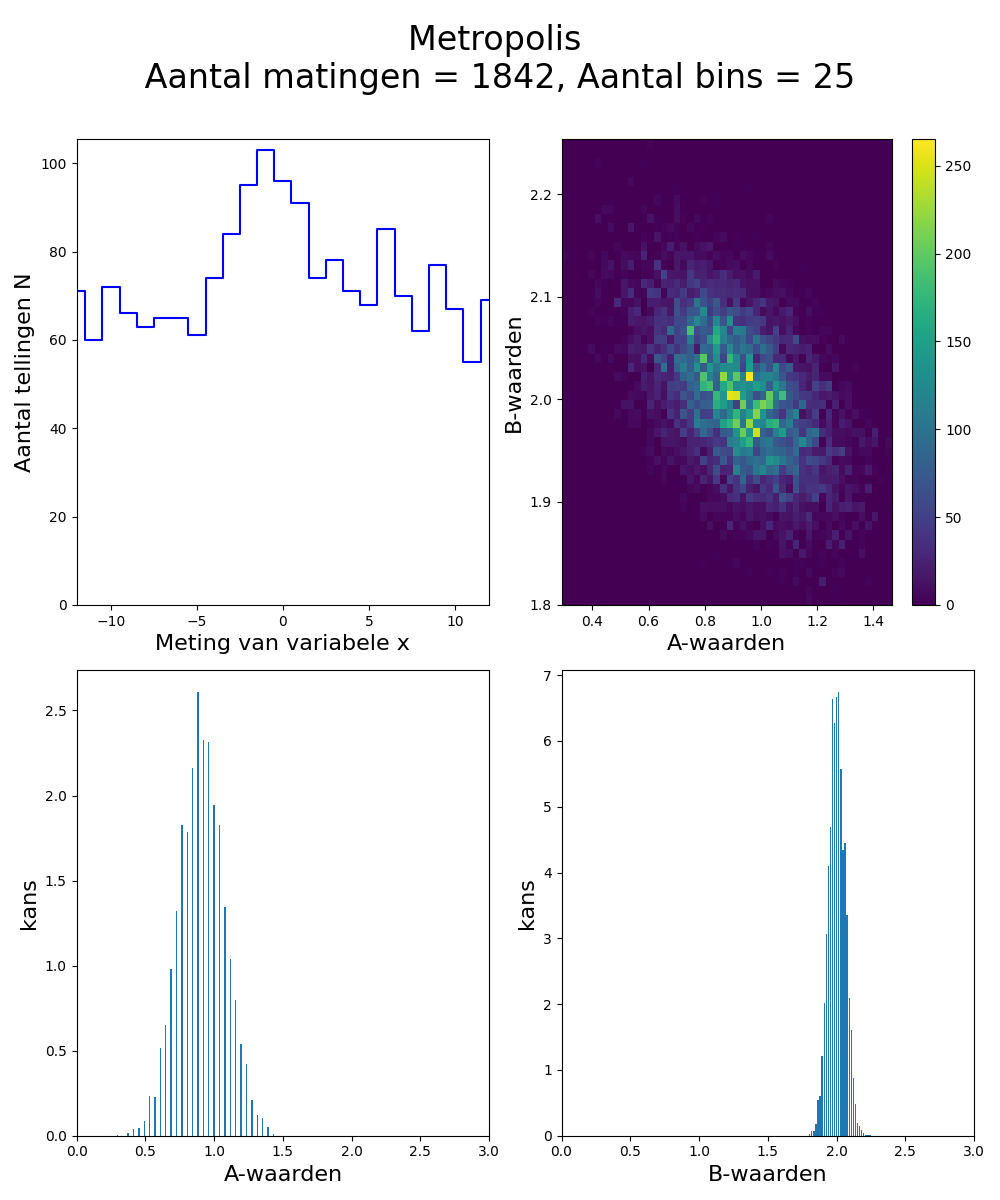
\includegraphics[width=0.95\linewidth]{Figures/signaal_AB_samples_100000.png}
        \subcaption{Figuren gegenereerd met het Metropolis algoritme.}
        \label{fig:AB-metropolis}
        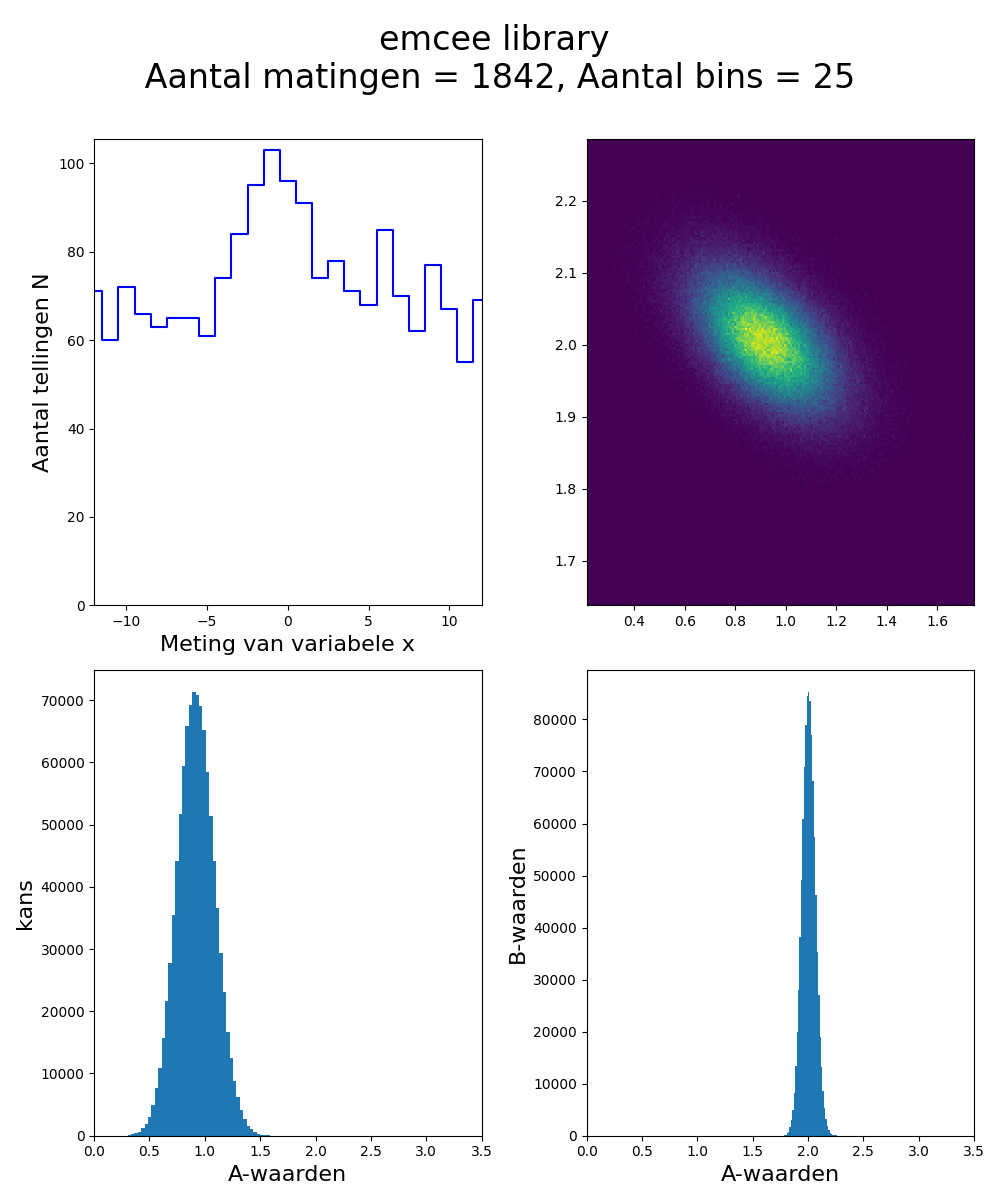
\includegraphics[width=0.95\linewidth]{Figures/emcee_hist_AB.png}
        \subcaption{Figuren met de emcee library.}
        \label{fig:AB-emcee}
    \end{minipage}
    \caption{Op de figuren staat exact hetzelfde als bij \cref{fig:AB-bay}. Hier werd er gewerkt met het Metropolis algoritme en de emcee library.  Het valt op dat de plots voor alle drie de manieren gelijkend zijn.}
    \label{fig:AB-met-mc}
\end{figure}\mbox{}\\
De figuren gegenereerd met het metropolis algoritme, met 1\_000\_000 metingen, waarvan er 60\_000 verwaarloosd zijn, zijn te vinden in \cref{fig:AB-metropolis}. \\ \\
De figuren gegenereerd met de emcee library zijn te vinden in \cref{fig:AB-emcee}. Hier werden 100 walkers gebruikt. Er werden 10\_000 datapunten gegenereerd, waarvan er 3\_000 weggegooid werden.
\\ \\
Er kan geconcludeerd worden dat de drie manieren van werken equivalente resultaten opleveren. De gevonden data is in de drie gevallen dezelfde, de pieken blijven op dezelfde plaats staan.
\subsection{Afschatten van de parameters van een sersic}
Voor het modelleren van het lichtintensiteitsprofiel van het helder sterrenstelsel wordt er gewerkt met een 2D-sersic
\cite{unknown-author-no-date-sersic}
\cite{wikipedia-contributors-2024}. Die 2D-sersic beschrijft hoe de intensiteit van een sterrenstelsel varieert met de afstand ten opzichte van het centrum. In formulevorm is dat dan gegeven door \cref{for: sersic}.
\begin{align}
    I(R)=I_{e}exp\left(b_{n}\left[\left(\frac{R}{R_{e}}\right)^{1/n}-1\right]\right)
    \label{for: sersic}
\end{align}
In \cref{for: sersic} is $I_{e}$ de amplitude, $b_{n}$ is een gammafunctie. $R_{e}$ is de effectieve straal, R is de afstand tot het middelpunt en n is de index van het profiel. Er wordt steeds gewerkt met index 1.\\ \\
Zo'n intensiteitsprofiel kan eenvoudig geplot worden met Python. Voor het plotten van een sersic moeten er zes parameters gekend zijn \cite{unknown-author-no-date-info-sersic};
\begin{enumerate}
    \item $x_{0}$: de $x$-positie van het middelpunt van het object
    \item $y_{0}$: de $y$-positie van het middelpunt van het object
    \item mate van ellipticiteit: een waarde tussen 0 en 1 waarbij 0 een cirkel is en 1 een parabool
    \item $r_{eff}$: de effectieve straal van het object, de straal waarbinnen de helft van het licht uitgestraald wordt \cite{wikipedia-contributors-2023-reff}
    \item amplitude: de helderheid van het object op een afstand $r_{eff}$ van het middelpunt
    \item $\theta$: de rotatiehoek van het object in radialen
\end{enumerate}
Stel al deze waarden zijn gekend, en zijn gelijk aan ($x_0$, $y_0$, ellips, $r_{eff}$, amplitude, $\theta$) = (100, 100, 0.3, 25, 1, $\frac{\pi}{4}$),
dan kan de 2D sersic getekend worden. Deze is te zien in \cref{fig: 2D_sersic}.
\begin{figure}
    \centering
    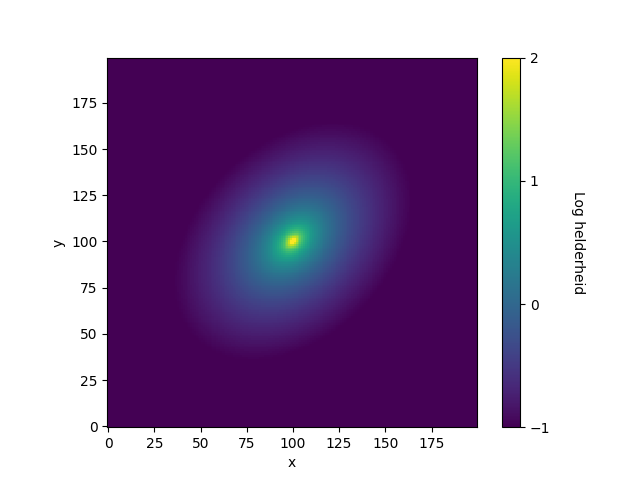
\includegraphics[width=0.95\linewidth]{Figures/figuur_2D_zonder_package_1_25_8_0.3_0.7853981633974483.png}
    \caption{Plot van een 2D sersic profiel met volgende parameters: ($x_0, y_0$, ellips, amplitude, $\theta$, $r_{eff}$) = (100,100,0.3,1,$\frac{\pi}{4}$,25).}
    \label{fig: 2D_sersic}
\end{figure}
Wat nu geprobeerd wordt is de afschatting van de zes parameters, gegeven een object. Hiervoor wordt opnieuw gebruik gemaakt van het Metropolis algoritme of van de emcee library. 
\subsubsection{De afschatting van de parameters van een sersic}
Om te beginnen wordt er gebruik gemaakt van het Metropolis algoritme. Om de complexiteit gradueel op te voeren wordt eerst enkel $x_{0}$ afgeschat, waarna ook $y_{0}$, de excentriciteit ... volgen. Wanneer niet alle parameters geschat worden, worden de resterende parameters als gekend beschouwd. Er wordt een dataset gesimuleerd op basis van de echte waarden van het object. Om de situatie meer waarheidsgetrouw te maken, wordt op de dataset poissonruis toegevoegd. Uit de posterior (die verteld hoe waarschijnlijk een combinatie van parameter is), wordt dan gesampled, in de hoop om de parameters van het object terug te vinden uit de dataset.
Er wordt gewerkt met volgende waarden voor de parameters: ($x_0$, $y_0$, ellips, $r_{eff}$, amplitude, $\theta$) = (16, 16, 0.35, 5, 50, $\frac{\pi}{4}$). \\ \\

De resultaten gebruikmakend van het Metropolis algoritme zijn te zien in \cref{appendix: opbouw}. Het eindresultaat, waarin alle zes de parameters afgeschat worden, is te zien in \cref{fig: 6 onbekenden}. Voor de afschatting van die zes parameters werden 9\_500\_000 samples gegenereerd waarvan er 1\_500\_000 weggegooid werden.
\begin{figure}
    \centering
    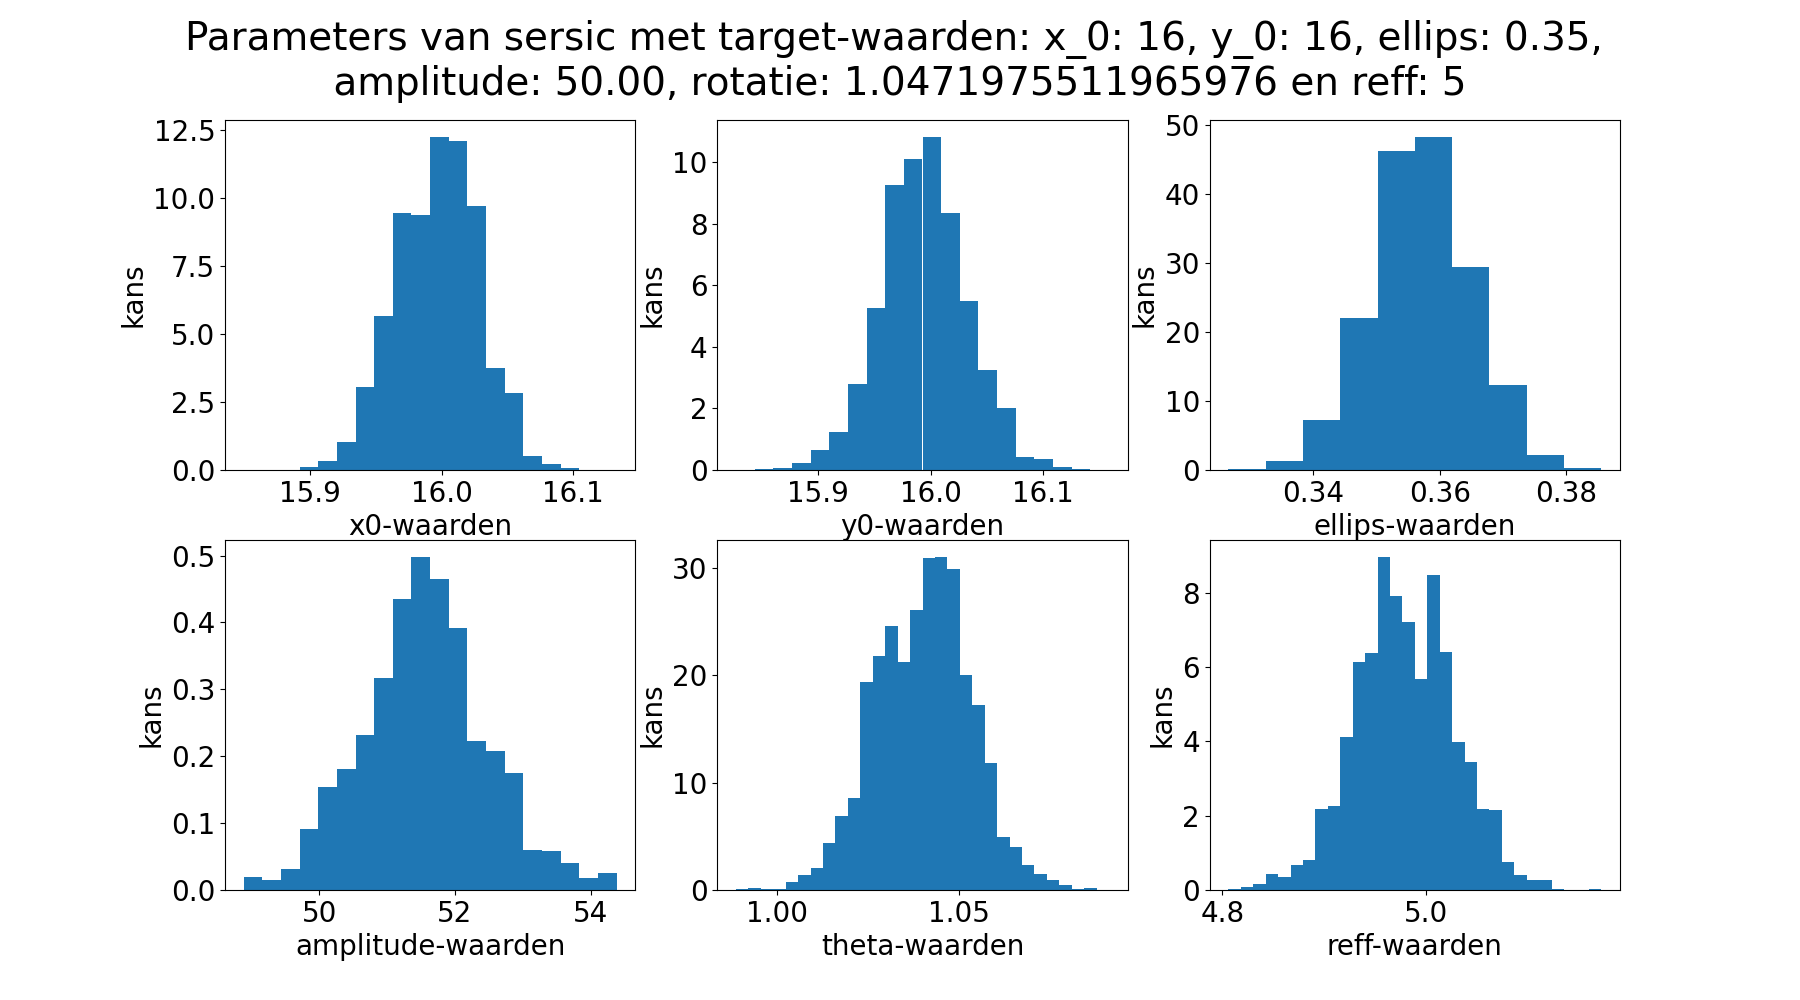
\includegraphics[width=0.95\linewidth]{Figures/sersic_parameters_metropolis_9500000_1500000_50_reff.png}
    \caption{Het resultaat van de afschatting van zes verschillende parameters van de sersic met waarden ($x_0,\ y_0$, ellips, amplitude, $\theta$, $r_eff$) = (16, 16, 0.35, 50, $\frac{\pi}{3}$,  5).}
    \label{fig: 6 onbekenden}
\end{figure}
Zoals te zien in \cref{fig: 6 onbekenden} komen de pieken van afgeschatte parameters goed overeen met de effectieve waarden die gebruikt zijn om de dataset te generen. \\ \\De afgeschatte parameters kunnen ook getoetst worden aan de bijhorende figuur van de sersic (opgebouwd op basis van de dataset die gemodelleerd is om de parameters af te schatten). Die figuur is te zien in \cref{fig: af te schatten sersic}. Op de figuur is inderdaad te zien dat de sersic ongeveer $45^{\circ}$ geroteerd is. Ook de $x_0$ en $y_0$ posities en de excentriciteit zijn te zien en komen inderdaad overeen met de waarden die afgeschat werden. 
\begin{figure}
    \centering
    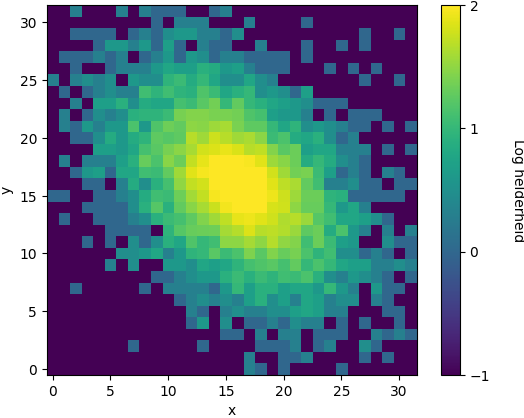
\includegraphics[width=0.95\linewidth]{Figures/sersic.png}
    \caption{Een 2D sersic gegenereerd volgens de dataset die gebruikt werd om de waarden van de sersic te zien in \cref{fig: 6 onbekenden} af te schatten.}
    \label{fig: af te schatten sersic}
\end{figure}\mbox{}\\ \\
Hetzelfde kan nu gedaan worden met behulp van de emcee library. Hier worden alle zes de parameters meteen tegelijk afgeschat. Het resultaat van de afschatting met 100 walkers, 12000 stappen, waarvan er 2300 weggegooid zijn, is te vinden in \cref{fig: emcee}.
\begin{figure}
    \centering
    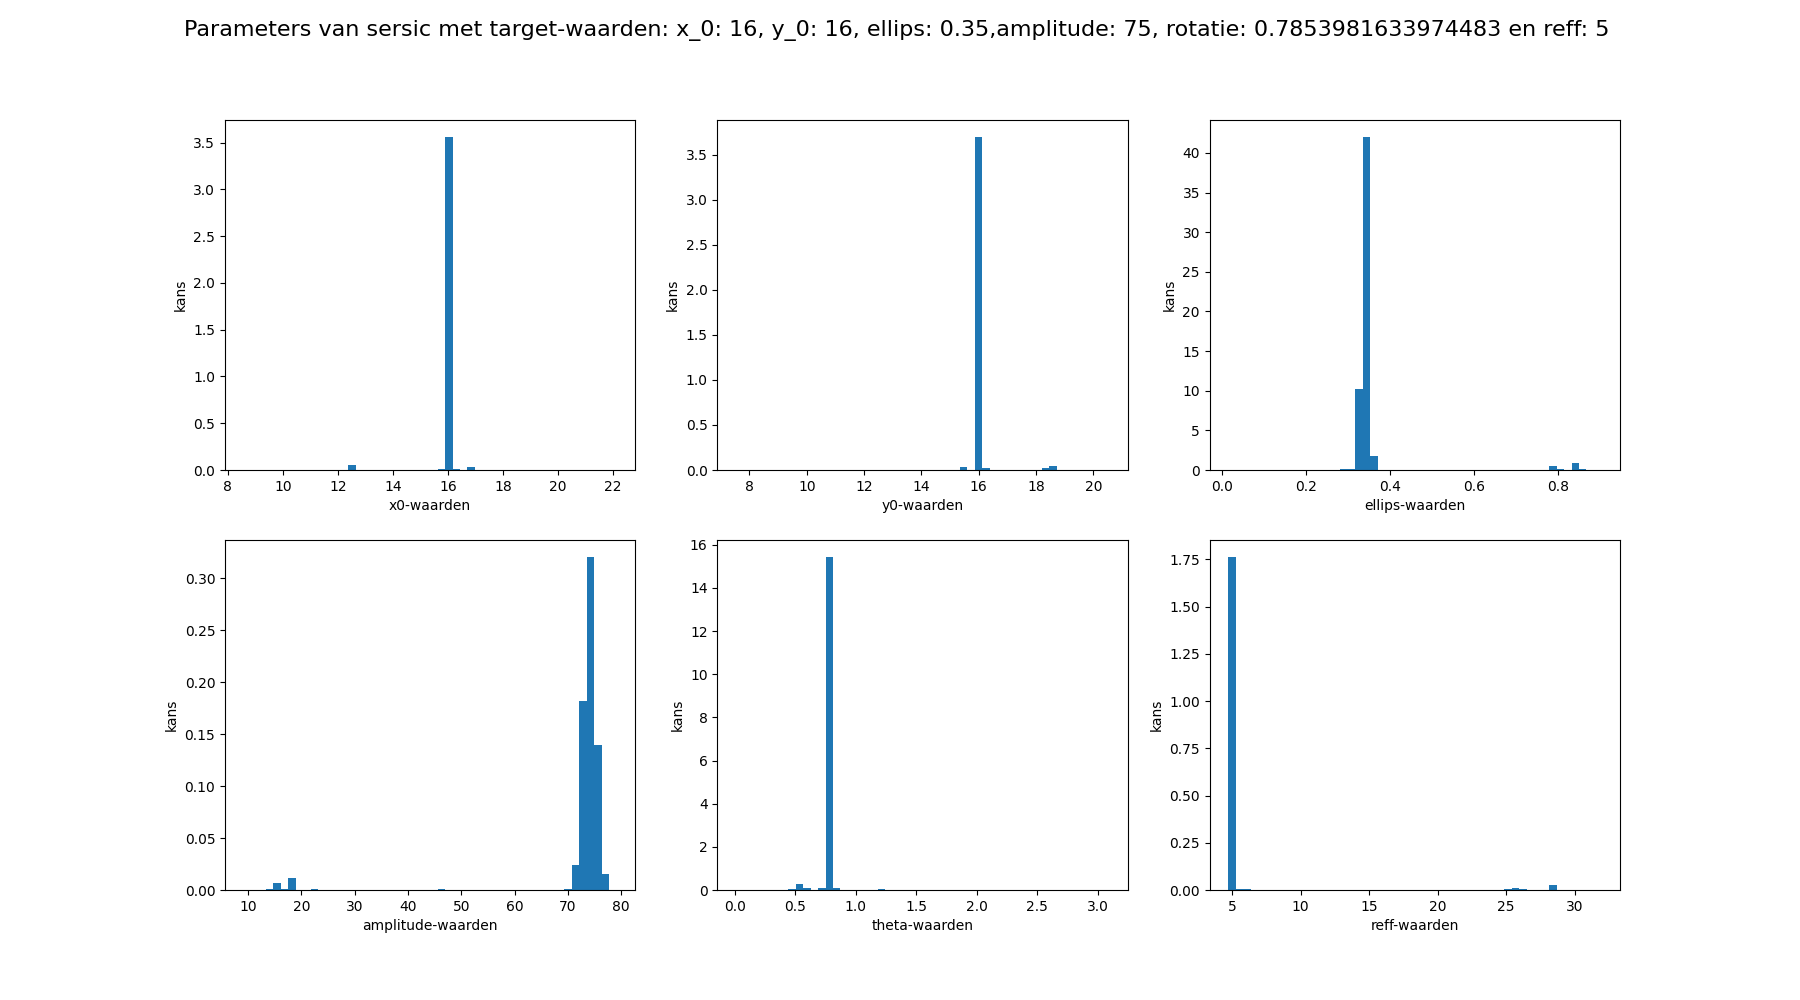
\includegraphics[width=0.95\linewidth]{Figures/emcee_hist_12000_2300.png}
    \caption{Het resultaat van het afschatten van de zes parameters van de sersic, gebruikmakend van de emcee library. De targetwaarden van deze sersic waren ($x_0,\ y_0$, ellips, amplitude, $\theta$, reff) = (16, 16, 0.35, 75, $\frac{\pi}{4}$,  5)}
    \label{fig: emcee}
\end{figure}\mbox{}\\
Opnieuw kan er een goede afschatting van de parameters van de sersic gemaakt worden. Werken met de emcee library blijft wel eenvoudiger, doordat er geen kennis van het systeem vereist is.

\subsection{Het afschatten van parameters van twee 2D sersic systemen}
Nu de parameters van één object afgeschat kunnen worden is het doel om ook de parameters van twee (of zelfs meerdere) objecten af te kunnen schatten. De werkwijze is volledig analoog aan het geval met slechts één object. Er wordt opnieuw gebruik gemaakt van zowel het Metropolis algoritme als de emcee library. \\ \\
Soms kan een object dat achter een ander object staat niet waargenomen worden. Dat wordt weergegeven in \cref{fig:2_sersic}. Daar staat op de eerste foto een eerste sersic, op de tweede foto staat een tweede sersic en op de derde foto zijn de beelden samengevoegd tot één afbeelding. \\ \\
Doordat een sersic soms verdwijnt achter een andere sersic is het nodig om de parameters van meerder objecten goed te kunnen schatten. Dit is nodig om verder te kunnen gaan in de bachelorproef. Er gaat later nog geprobeerd worden om de achtergrond waarop het sersicsysteem staat af te schatten, en dan is het belangrijk dat ook systemen met meerdere sersics afgeschat kunnen worden. 
\begin{figure}
    \centering
    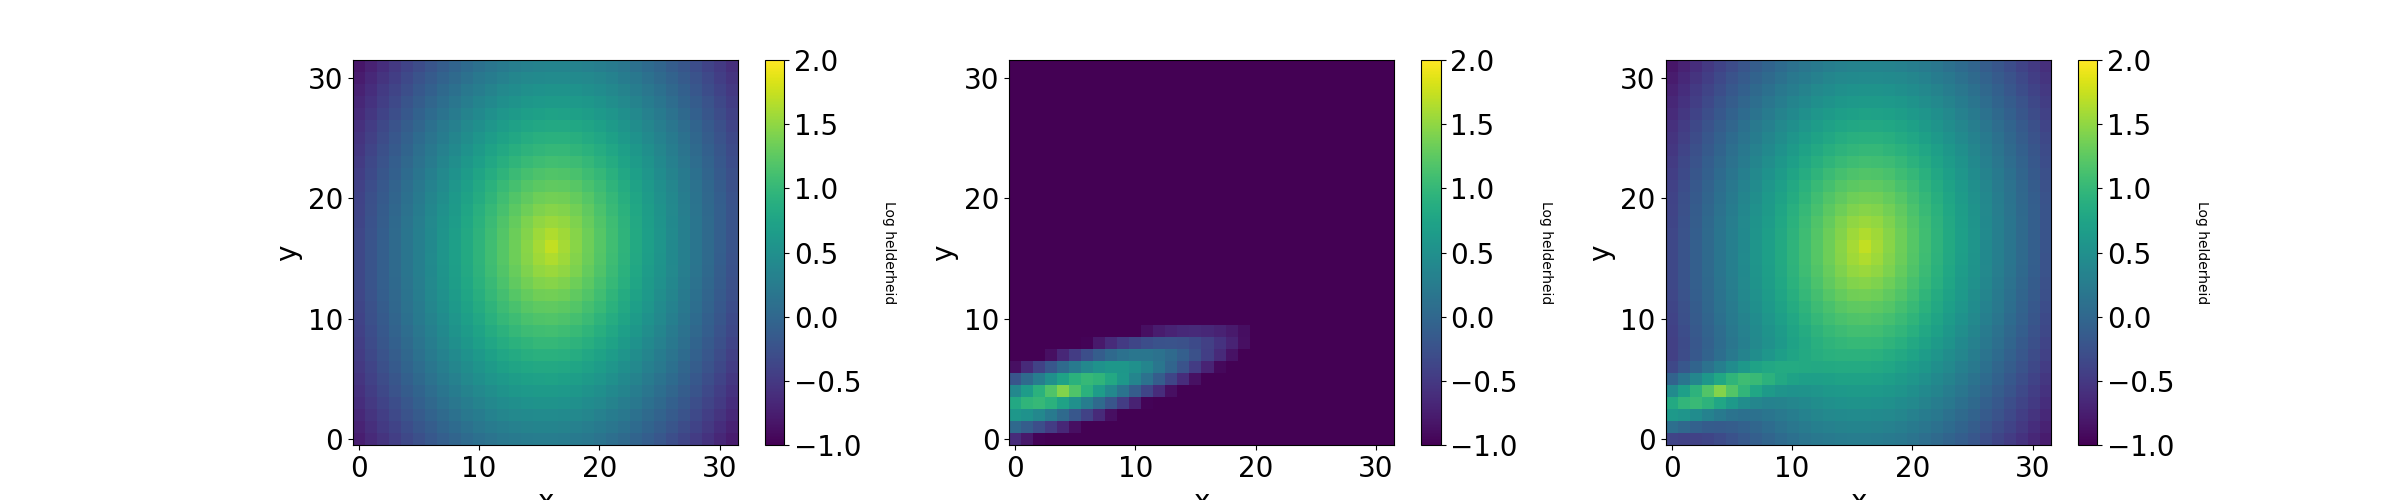
\includegraphics[width=0.99\linewidth]{Figures/figuur_2D_zonder_package_10_8_1_0.3_1.5.png}
    \caption{Op de meest linkse figuur staat een heldere sersic, op de middelste figuur staat een tweede, over het algemeen minder heldere sersic. Op de meest rechtse figuur is het resultaat van de optelling van de twee sersics te zien.}
    \label{fig:2_sersic}
\end{figure}\mbox{}\\
Er werd een eerste poging gedaan tot het afschatten van de parameters van de twee sersic profielen. De resultaten ervan zijn te zien in \cref{fig:sersic 1} en \cref{fig:sersic 2} voor respectievelijk de eerste sersic en de tweede. Wat opvalt is dat er op beide figuren twee pieken staan. Dat is logisch, doordat er ontaarding is. Het algoritme kan niet bepalen welke sersic nummer 1 is, en welke sersic nummer 2 is. De afgeschatte waarden komen overeen met wat er verwacht wordt, maar het is nu nog zaak om de juiste parameters te koppelen aan de juiste sersic.
\\ \\
In het proces van het genereren van de samples wordt er steeds een voorstel gedaan, een kans bepaald, en dan wordt een staat geaccepteerd of verworpen. Er wordt vanaf nu bijgehouden welke combinatie van parameters de hoogste kans had (hoewel het eigenlijk strikt genomen over kansdichtheden gaat). Dan is nog niet geweten welke set van parameters sersic 1 beschrijft, en welke set van parameters sersic 2 beschrijft, maar dat hoeft geen probleem te zijn. De juiste combinaties van de parameters is dan wel gekend. Het resultaat is te zien in \cref{fig: 2 sersic niet ontaard}.
\begin{figure}
    \begin{minipage}{0.98\linewidth}
        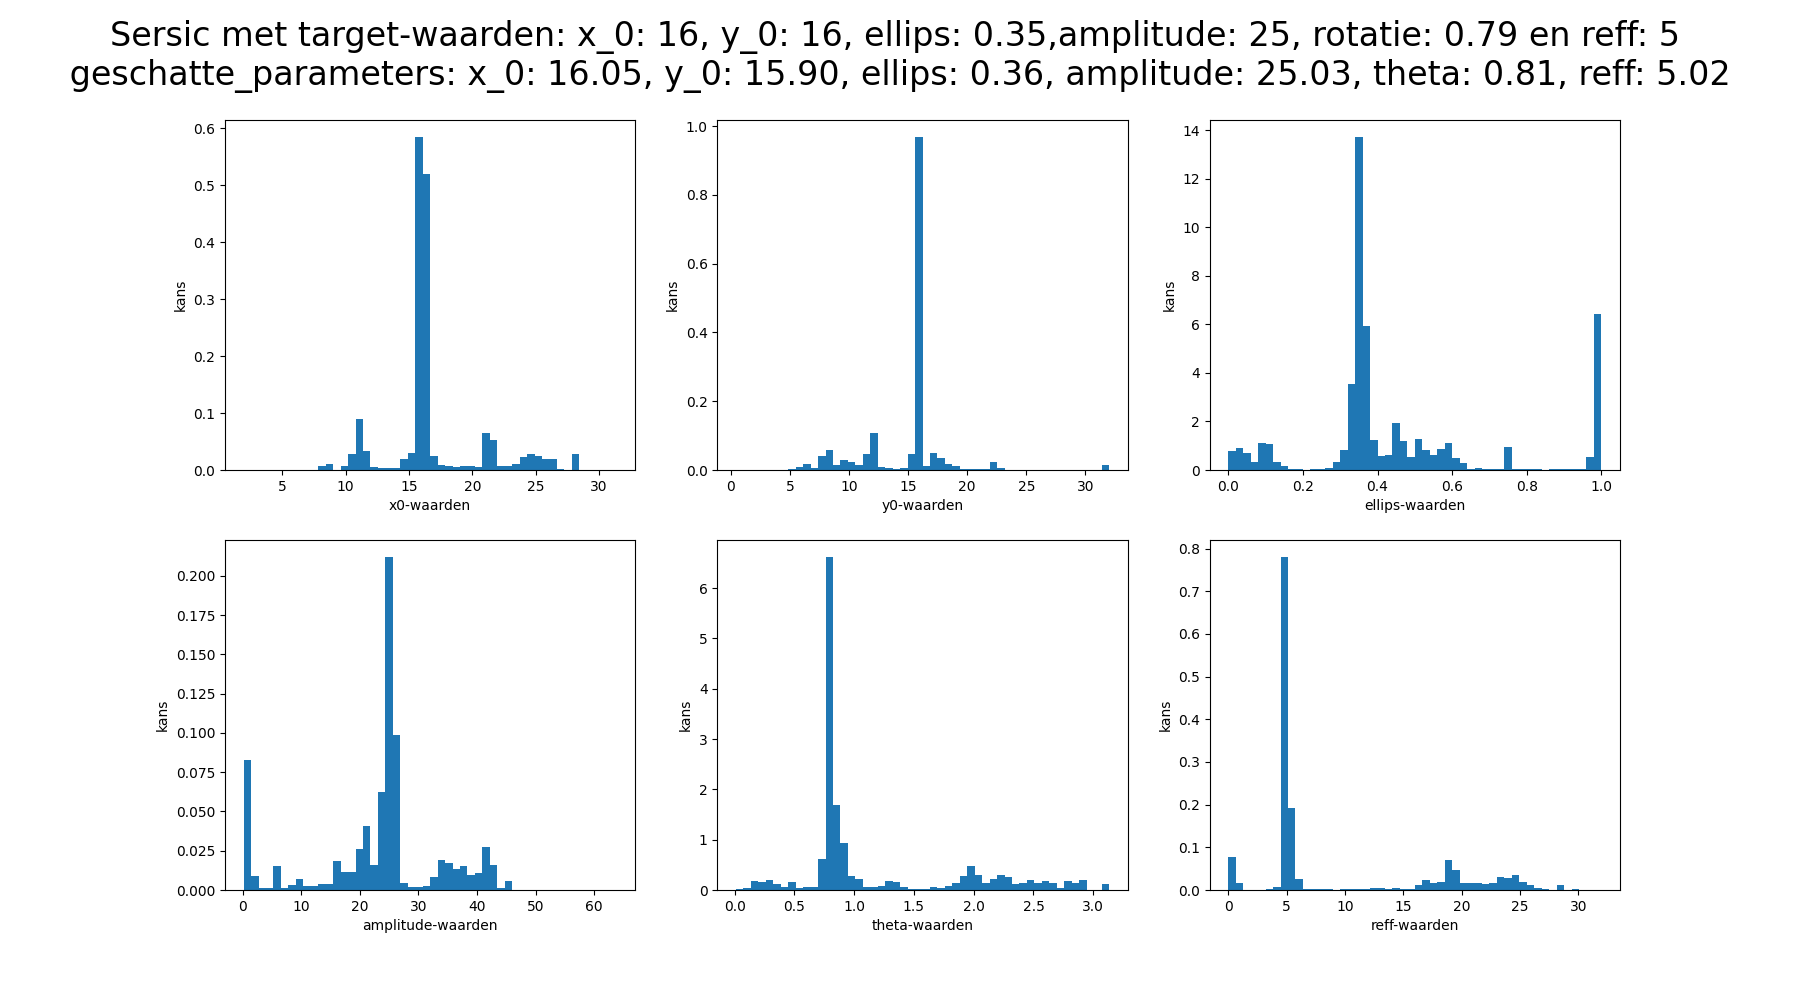
\includegraphics[width=0.95\linewidth]{Figures/1_emcee_hist_5000_750.png}   
        \subcaption{De parameters van de eerste van twee sersics}
        \label{fig:sersic 1}
        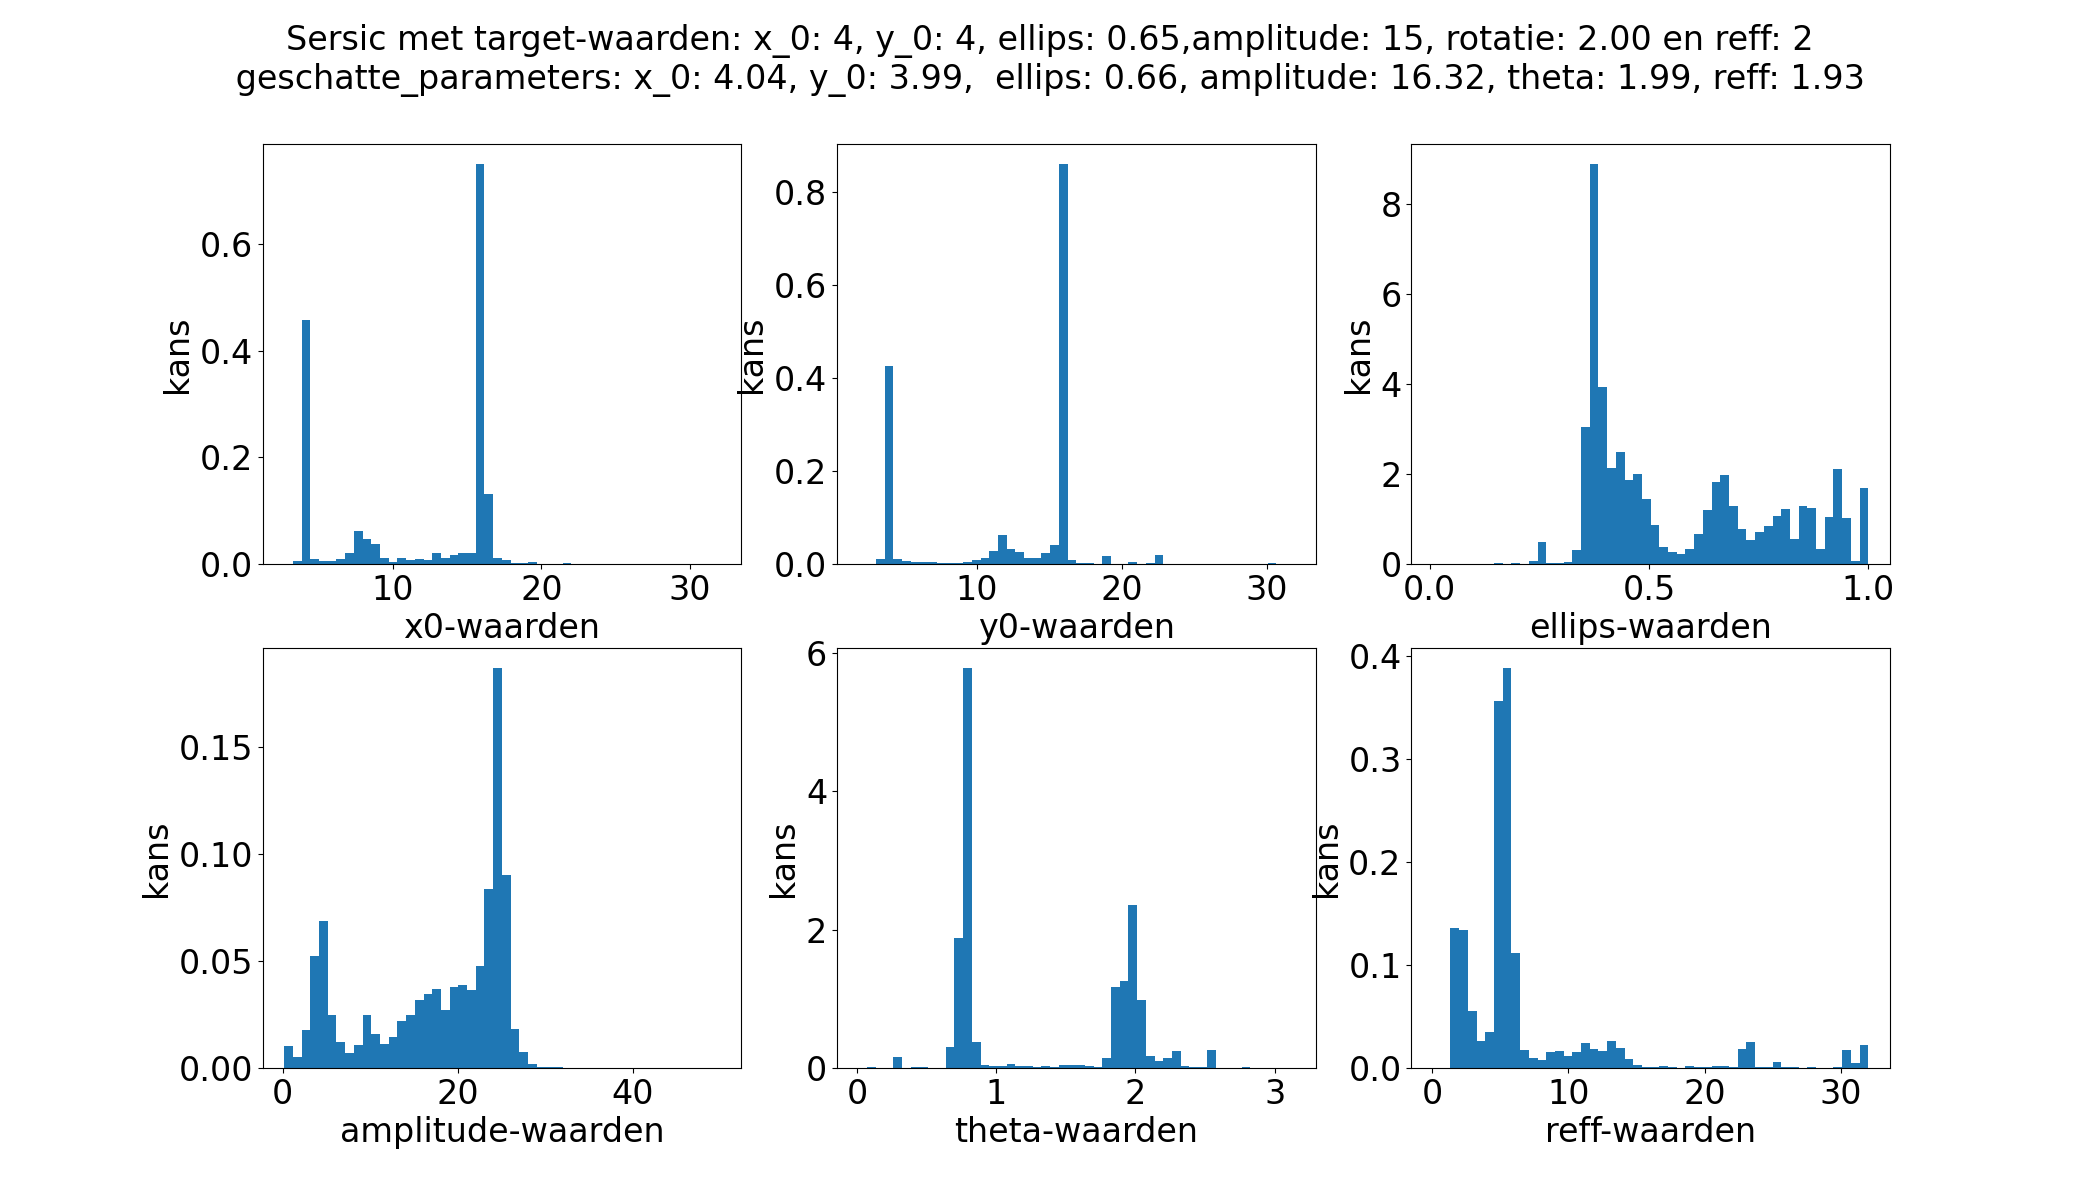
\includegraphics[width=0.95\linewidth]{Figures/2_emcee_hist_5000_750.png}
        \subcaption{De parameters van de tweede sersic}
        \label{fig:sersic 2}
        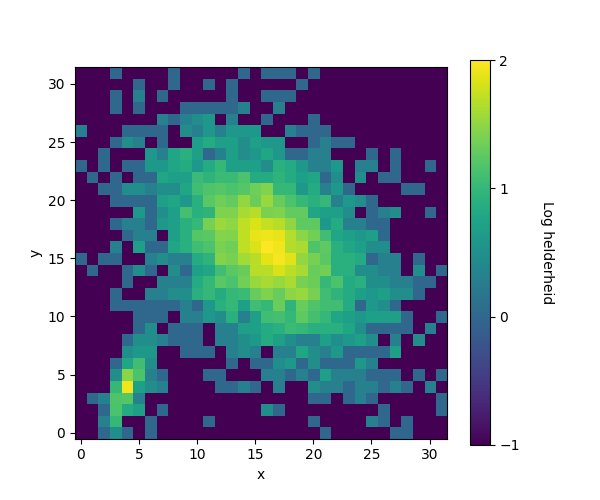
\includegraphics[width=0.95\linewidth]
        {Figures/figuur_2D_zonder_package_5000.png}
        \subcaption{Een plot van het sersicsysteem volgens de gegenereerde data.}
    \end{minipage}
    \caption{De afschatting van de parameters in het geval van twee sersic (waarbij de ene sersic naast de andere staat) in dezelfde figuur. Naast de verwachte parameters worden ook steeds de geschatte parameters weergegeven. Ook de plot van de af te schatten sersic wordt weergegeven. Op de grafieken is nog steeds ontaarding te zien, maar het koppelen van de juiste parameters lukt door gebruik te maken van onze methode van de grootste kans}
    \label{fig: 2 sersic niet ontaard}
\end{figure}
De parameters van beide sersics kunnen goed afgeschat worden. Op deze manier kan het totale sersicstelsel goed afgeschat worden. In de laatste stap van deze bachelorproef wordt er geprobeerd om de parameters van een sersic af te schatten zodat de achtergrond waarop deze sersic staan gevonden kan worden. Het is dan ook belangrijk dat eender welk sersicsysteem (ook een systeem met meerdere sersics) goed afgeschat kan worden.

\subsection{De afschatting van parameters van een 2D sersic systeem met een werkelijke achtergrond}
In de voorgaande bepaling van de parameters van het sersic profiel werd aan de dataset van de werkelijke waarden wat ruis toegevoegd. Nu wordt overgegaan op een meer werkelijke toestand door de sersic met het poissonruis te plaatsen op een achtergrond die gemodelleerd is door NASA. \\ \\
De achtergrond die gebruikt wordt is te zien in \cref{fig:NASA}. Dit is een zeer grote foto, voor de achtergrond in het programma werd een deeltje van 64x64 pixels genomen uit deze afbeelding. Zo'n figuur is te zien in \cref{fig:achtergrond nasa}.
Hierop werd dan een sersic geplaatst om zo tot een nieuw geheel te komen. Zo'n sersic op de werkelijke achtergrond is te zien in \cref{fig:achtergrond+sersic}. Dit zal uiteindelijk ook de dataset worden.
\begin{figure}
    \begin{minipage}{0.98\linewidth}
        \centering
       \includegraphics[width=0.55\linewidth]{Figures/achtergrond_groot.jpg}
        \subcaption{Een achtergrondbeeld gemodelleerd door NASA. Foto van \cite{nasa-2023}}
        \label{fig:NASA} 
        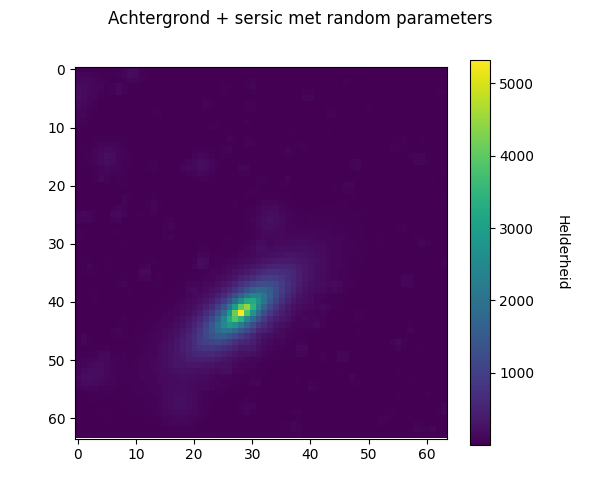
\includegraphics[width=0.85\linewidth]{Figures/sersic+achtergrond_656679_clip2.png}
        \caption{Een 2D sersic profiel op een werkelijke achtergrond.}
        \label{fig:achtergrond+sersic}
    \end{minipage}
    \caption{De opbouw van het genereren van een sersic op een werkelijke achtergrond. Eerst wordt een deeltje geknipt uit de werkelijke achtergrond (zie \cref{fig:achtergrond nasa}), er wordt een sersic gegeneerd met willekeurige parameters. De sersic wordt opgeteld bij de achtergrond en geeft zo een ruizig geheel dat de werkelijkheid weerspiegeld.}
\end{figure}
\\
Het uiteindelijke doel is nu om de waarden van de sersic af te schatten om zo enkel de achtergrond te bekomen. De afschatting van de parameters van deze sersic wordt gedaan door gebruik te maken van de emcee library.
\\ \\

Vanuit het geheel (een sersic met poissonruis geplaatst op een achtergrond) worden nu de parameters van de sersic afgeschat. Als de parameters geschat zijn wordt een afgeschatte sersic getekend (op basis van de geschatte parameters). Om dan de achtergrond te vinden wordt de geschatte sersic afgetrokken van het geheel. Zo blijft enkel de achtergrond over. De achtergrond geknipt uit het beeld van NASA is te zien in \cref{fig:achtergrond nasa}, het totaal is te zien in \cref{fig:achtergrond+sersic} en de afgeschatte achtergrond is te zien in \cref{fig:geschatte achtergrond}.
\\ \\
\begin{figure}
    \begin{minipage}{0.98\linewidth}
        \centering
        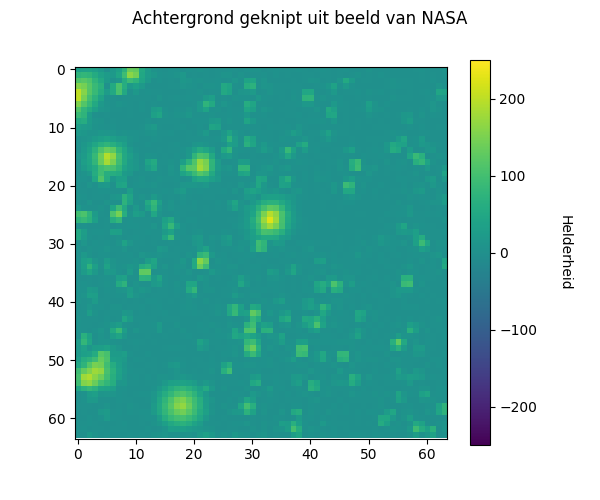
\includegraphics[width=0.95\linewidth]{Figures/sersic_achtergrond_656679_clip2.png}
        \subcaption{De achtergrond geknipt uit de gemodelleerde achtergrond van NASA}
        \label{fig:achtergrond nasa}
        \centering
        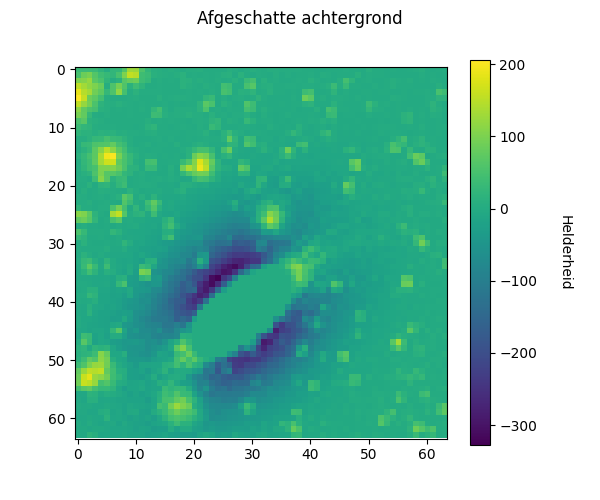
\includegraphics[width=0.95\linewidth]{Figures/afgeschatte_achtergrond_656679.png}
        \subcaption{De afgeschatte achtergrond, waarin de zes parameters van de sersic afgeschat werden.}
        \label{fig:geschatte achtergrond}
    \end{minipage}
    \caption{De vergelijking tussen de oorspronkelijke achtergrond (\cref{fig:achtergrond nasa}) de afgeschatte achtergrond (\cref{fig:geschatte achtergrond}). De sersic geplaatst op de achtergrond is te zien in \cref{fig:achtergrond+sersic}. Over het algemeen komen de figuren goed overeen, maar op de afgeschatte achtergrond is wel duidelijk te zien dat sersic niet volledig correct afgeschat is.}
\end{figure}

Op de figuren is te zien dat de afgeschatte achtergrond wel goed overeenkomt met de werkelijke achtergrond. Wat wel opvalt is dat de parameters van de sersic niet zo goed afgeschat zijn. Daardoor blijft een deel van de sersic zichtbaar en zijn we nog niet in staat om de objecten achter de sersic te zien. \\ \\
Wat verder ook opvalt is dat er sommige plaatsen teveel afgetrokken wordt van de figuur, op andere plaatsen wordt er te weinig afgetrokken. Er werd geprobeerd om ervoor te zorgen dat er nooit te veel afgetrokken zou kunnen worden, waardoor er geen negatieve waarden bekomen konden worden. Dit werkte echter niet, er werd geen enkele combinatie van waarden meer gevonden. \\ \\
In de toekomst zou het afschatten van de achtergrond ook met AI kunnen gebeuren. Er is al een dataset die bestaat uit 100 sets van de sersic + achtergrond enerzijds, en de achtergrond anderzijds. Met deze dataset zou een AI getraind kunnen worden.











\section{CONCLUSIE}
% Edit below
Er kan geconcludeerd worden dat zowel de stelling van Bayes, het Metropolis algoritme en de emcee library leiden tot goede resultaten. De parameters van een sersicsysteem bestaande uit één sersic konden afgeschat worden. Ook de parameters van een systeem met twee sersics konden afgeschat worden. Op die manier kan er info bekomen worden van het beeld achter de zware massa. Ook werd er geprobeerd om van een sersic op een werkelijke achtergrond de parameters van de sersic af te schatten om zo de achtergrond te reconstrueren. Dit zou gebruikt kunnen worden om een AI te trainen, die dan zelf de sersic van de achtergrond zou kunnen halen om de achtergrond zelf te reconstrueren. \\ \\
Het afschatten van de waarden van de sersic op de werkelijke achtergrond ging niet zo goed, vermoedelijk doordat de werkelijke achtergrond veel ruiziger is dan de poissonruis die toegevoegd werd aan de sersic in de eerdere afschattingen. Er werd geprobeerd om er voor te zorgen dat er geen negatieve waarden gegenereerd konden worden. Dit is niet gelukt, er werden geen goede waarden meer gevonden.

% Additional sections for acknowledgments
\rule{\linewidth}{0.4pt}
\textit{Author contributions}
% Edit below
JL heeft het onderzoek bedacht en vorm gegeven.
YR heeft de algoritmes geschreven en er experimenten mee gedaan. \\ \\
\textit{Acknowledgements} 
YR bedankt JL voor de begeleiding en ondersteuning. \\ \\
\textit{Beschikbaarheid van data en code}
De data en code die bij het maken van dit artikel gebruikt werden, worden op verzoek beschikbaar gesteld door de corresponderende auteur.
% Edit below
\newpage
\newpage
\appendix
\addcontentsline{toc}{section}{Appendices}
\section*{Appendices}
\section{Newtoniaanse bepaling afbuighoek als gevolg van een gravitationeel veld}
\label{appendix: newton}
Er wordt vertrokken vanuit de bewegingsvergelijkingen voor een deeltje in een potentiaal, gecreëerd door het zwaartekrachtveld. Er wordt aangetoond dat de oplossingen van de bewegingsvergelijking kegelsneden (cirkel, ellips, hyperbool, parabool) als oplossing heeft. Deze afleiding is gebasserd op het handboek Analytical Mechanics van Hand en Finch, \cite{hand-1998}.
\subsection{De baan van een deeltje in een zwaartekrachtveld zijn kegelsneden}
Voor gravitatie wordt de potentiële energie gegeven door
$$V(r)=-\frac{GmM}{r}$$
De effectieve potentiële energie is gegeven door
$$V_{eff}(r)=-\frac{k}{r}+\frac{l^{2}}{2\mu r^{2}}$$
Hierin is $k=GmM$.\\
$\mu$ is de gereduceerde massa, deze wordt gevonden uit $\frac{1}{\mu}=\frac{1}{M}+\frac{1}{m}$\\
De bewegingsvergelijking wordt dan gegeven door
$$\mu\ddot{r}=\frac{l^{2}}{\mu r^{3}}-\frac{k}{r^{2}}$$
Deze vergelijking is niet lineair. We voeren een nieuwe variabele in. Stel $u=\frac{1}{r}$ en $\dot{\phi}=\frac{l}{\mu r^{2}}$, dit volgt uit behoud van draaimoment. We weten dan dat
$$\mu r^{2}\dot{\phi}=l;\ \ \ \ \ \mu r^{2}d\phi=ldt;\ \ \ \ \ dt=\frac{\mu}{lu^{2}}d\phi$$
Dan geldt er dat
\begin{align}
\dot{r}&=\frac{d}{dt}r=\frac{d}{dt}\left(\frac{1}{u}\right) \nonumber \\
&=-\frac{1}{u^{2}}\frac{du}{dt} \nonumber \\
&=-\frac{1}{u^{2}}\frac{du}{d\phi}\frac{d\phi}{dt} \nonumber \\
&=-\frac{1}{u^{2}}\frac{lu^{2}}{\mu}\frac{du}{d\phi} \nonumber \\
&=-\frac{l}{\mu}\frac{du}{d\phi} \nonumber 
\end{align}
De 2de afgeleide is gegeven door
\begin{align}
\ddot{r}&=\frac{d}{dt}\left[-\frac{l}{\mu}\frac{du}{dt}\right] \nonumber \\
&=-\frac{l}{\mu}\frac{d}{d\phi}\left(\frac{du}{d\phi}\right)\frac{d\phi}{dt} \nonumber \\
&=-\frac{l}{\mu}\frac{lu^{2}}{\mu}\frac{d^{2}u}{d\phi^{2}} \nonumber 
\end{align}
Dan krijgen we als differentiaalvergelijking van de baan dat
$$\frac{d^{2}u}{d\phi^{2}}+u=\frac{k\mu}{l^{2}}$$
De oplossing van deze differentiaalvergelijking is gegeven door
$$u(\phi)=\frac{\mu k}{l^{2}}+A\cos(\phi)$$
We gaan nu overgaan op Cartesische coördinaten. Stel $p=\frac{l^{2}}{\mu k}$ en stel $\epsilon=pA\geq0$. Dan geldt er
$$pu=1+\epsilon\cos(\phi)$$
$$p=r+r\epsilon \cos(\phi)$$
$$(p-\epsilon x)^{2}=x^{2}+y^{2}$$
De energie is gegeven door
\begin{align}
    E&=\frac{1}{2}\mu(\dot{r}^{2}+r^{2}\dot{\phi}^{2})-\frac{k}{r}\nonumber \\
    &=\frac{\mu k^{2}}{2l^{2}}(\epsilon^{2}-1)
    \label{for: energie}
\end{align}
Merk op dat de energie afhankelijk is van $\epsilon$. 
\begin{itemize}
\item  $\epsilon=0$: we hebben een minimum van de energie. Er geldt
$$x^{2}+y^{2}=p^{2}$$
Dit is exact gelijk aan de vergelijking van een cirkel met als straal p. Deze straal is exact gelijk aan het minimum van $V_{eff}$. 
\item $\epsilon=1$, dan is de energie gelijk aan 0. De baan is dan gegeven door
$$p^{2}+x^{2}-2px=x^{2}+y^{2}$$
$$2px=p^{2}-y^{2}$$
$$x(y)=\frac{p^{2}-y^{2}}{2p}$$
Dit is de baan van een parabool
\item $0<\epsilon<1$, dit komt overeen met een energie die kleiner is dan 0. De baan is dan gegeven door
$$p^{2}+\epsilon^{2}x^{2}-2\epsilon px-x^{2}-y^{2}=0$$
$$\left(1-\epsilon^{2}\right)x^{2}+2\epsilon px+y^{2}-p^{2}=0$$
\begin{align}
    &\left(1-\epsilon^{2}\right)\left(x^{2}+\frac{2\epsilon px}{(1-\epsilon^{2})}+\frac{\epsilon^{2}p^{2}}{(1-\epsilon^{2})^{2}} \frac{\epsilon^{2}p^{2}}{(1-\epsilon^{2})^{2}}\right)\nonumber \\
    &+y^{2}-p^{2}=0    \nonumber
\end{align}
$$\left(1-\epsilon^{2}\right)\left(x+\frac{\epsilon p}{(1-\epsilon^{2})}\right)^{2}+y^{2}-\frac{\epsilon^{2}p^{2}}{(1-\epsilon^{2})}-p^{2}=0$$
$$\left(1-\epsilon^{2}\right)\left(x+\frac{\epsilon p}{(1-\epsilon^{2})}\right)^{2}+y^{2}=\frac{p^{2}}{(1-\epsilon^{2})}$$
Dit kunnen we ook nog schrijven als
$$\frac{(x-x_{c})^{2}}{a^{2}}+\frac{y^{2}}{b^{2}}=1$$
Met: \\
$x_{c}=\frac{-\epsilon p}{1-\epsilon^{2}}$ \\
$p=\frac{l^{2}}{\mu k}$\\
$\epsilon = pA$\\
$a=\frac{p}{1-\epsilon^{2}}$\\
$b=\frac{p}{\sqrt{1-\epsilon^{2}}}$\\
Dit komt overeen met de baan van een ellips
\item $\epsilon > 1$, dit komt overeen met een energie die groter is dan 0. 
$$\frac{(x-x_{c})^{2}}{a^{2}}-\frac{y^{2}}{b^{2}}=1$$
Dit is de baan van een hyperbool
\end{itemize}
\subsection{De bijhorende afbuighoek voor een hyperbolische baan}
De verandering in kinetische energie van het deeltje met massa $m$ en snelheid $v$ in de potentiaal (per eenheidsmassa) is gegeven door 
\begin{equation}
    E=\frac{1}{2}mv^{2}
    \label{for:energie}
\end{equation}
Het draaimoment per eenheidsmassa is gegeven door
\begin{equation}
    L=bv
    \label{for:draaimoment}
\end{equation}
Deze twee grootheden kunnen ook geschreven worden in termen van de excentriciteit. Vertrekende van de energie gevonden in \cref{for: energie}, en gebruikmakende van $p=\frac{l^{2}}{\mu k}$ vinden we
$$E=\frac{k}{2p}(\epsilon^{2}-1)$$
We definiëren nu a als
$$a=\frac{p}{\epsilon^{2}-1}$$
Zo vinden we dan voor de energie per eenheidsmassa dat
\begin{align}
    E &= \frac{k}{2ma}\nonumber \\
    &= \frac{GM}{2a}
    \label{for:E}
\end{align}
Voor het draaimoment per eenheidsmassa geldt
\begin{align}
    L^{2} &= r^{2}v^{2}\nonumber \\
    &= r^{2}\cdot 2E \nonumber \\
    &= \frac{GM}{a}\cdot b^{2}
    \label{for:L2}
\end{align}
\begin{figure}
    \centering
    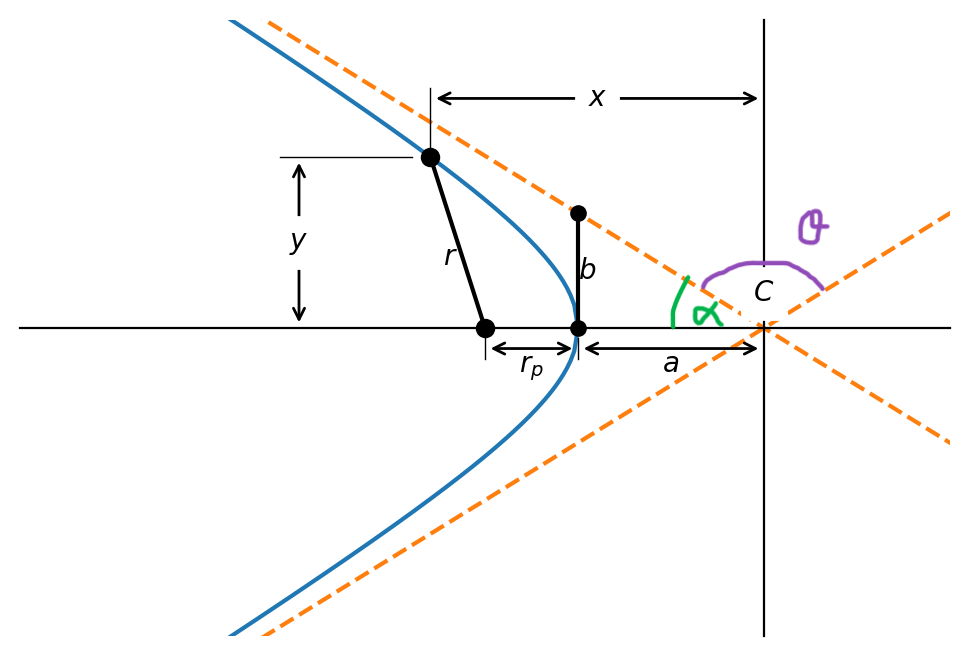
\includegraphics[width=0.95\linewidth]{Figures/hoek_hyperbool.png}
    \caption{De halve hoek van een hyperbolische baan. Figuur van Weber, \cite{weber-no-date}}
    \label{fig: halve hoek}
\end{figure}
De halve hoek van de hyperbolische baan is te zien in \cref{fig: halve hoek}. Daaruit volgt eenvoudig dat:
\begin{equation}
    tan(\alpha) = \frac{b}{a}
    \label{for: hoek}
\end{equation}
We gaan \cref{for: hoek} herschrijven in termen van L (\cref{for:L2}) en E (\cref{for:E}).
Merk op dat
$$E\cdot L^{2}=\frac{G^{2}M^{2}b^{2}}{2a^{2}}$$
$$\frac{2E\cdot L^{2}}{G^{2}M^{2}}=\frac{b^{2}}{a^{2}}$$
$$\frac{\sqrt{2E}L}{GM}=\frac{b}{a}$$
Invullen van \cref{for:energie} en \cref{for:draaimoment} geeft
\begin{align}
    \frac{b}{a}&=\frac{\sqrt{2\cdot\frac{1}{2}v^{2}}rv}{GM}\nonumber \\
     &= \frac{rv^{2}}{GM}\nonumber\\
\end{align}
Voor de hoek vinden we dan
\begin{equation}
    \tan(\alpha) =\frac{rv^{2}}{GM} 
    \label{for:tangens}
\end{equation}
De afbuighoek is gegeven door de hoek tussen de asymptoten. Als we kijken op \cref{fig: halve hoek} dan zien we
$$\theta = \pi - 2\alpha$$
Omvormen naar $\alpha$ geeft
$$\alpha = \frac{\pi}{2}-\frac{\theta}{2}$$
De tangens nemen
\begin{equation}
    \tan(\alpha) = \tan\left(\frac{\pi}{2}-\frac{\theta}{2}\right)
    \label{for:tan}
\end{equation}
We herschrijven de laatste tangens:
\begin{align}
    \tan\left(\frac{\pi}{2}-\frac{\theta}{2}\right)&=\frac{\sin(\frac{\pi}{2}-\frac{\theta}{2})}{\cos(\frac{\pi}{2}-\frac{\theta}{2})}\nonumber\\
    &= \frac{\cos(\frac{\theta}{2})}{\sin(\frac{\theta}{2})}\nonumber \\
    & = \cot(\frac{\theta}{2})
    \label{for:cot}
\end{align}
Invullen van \cref{for:cot} in \cref{for:tan} geeft
\begin{equation}
    tan(\alpha) = \frac{1}{tan(\frac{\theta}{2})}
    \label{for:afbuighoek}
\end{equation}
Invullen van \cref{for:tangens} en Taylor toepassen voor kleine $\theta$
$$\frac{1}{tan(\frac{\theta}{2})} = \frac{rv^{2}}{GM}$$
$$\frac{1}{\frac{\theta}{2}}=\frac{rv^{2}}{GM}$$
$$\frac{\theta}{2} = \frac{GM}{rv^{2}}$$
$$\theta = \frac{2GM}{rv^{2}}$$
Als de afbuiging van licht beschouwd wordt is de snelheid gegeven door de snelheid van het licht. Dan is de afbuighoek gegeven door \cref{for: afbuighoek}.
\begin{equation}
    \theta = \frac{2GM}{rc^{2}}
    \label{for: afbuighoek}
\end{equation}
Dit was nu de afleiding voor de hyperbool. Merk op dat dit de Newtoniaanse afleiding was. Als de gravitationele correcties mee in rekening gebracht worden, wordt in de teller een extra factor 2 gevonden.
\section{De lensvergelijking}
\label{appendix:lensvergelijking}
De werking van de lens kan benaderd worden als een geometrisch probleem in twee dimensies. De voorstelling van de werking van de lens is te zien in \cref{fig:lensvgl}
\begin{figure}[H]
    \centering
    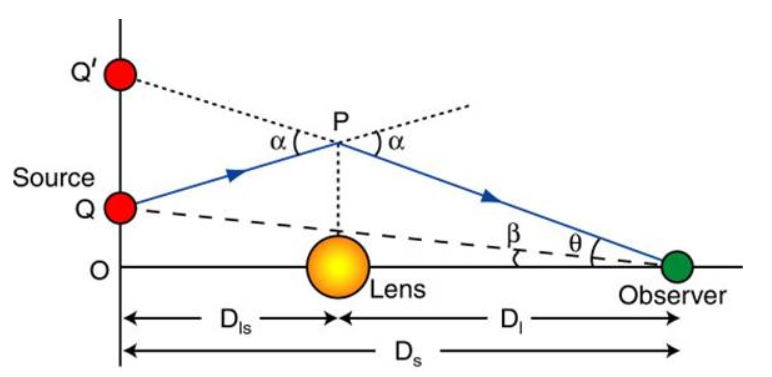
\includegraphics[scale=0.5]{Figures/Lensvergelijking.png}
    \caption{Schets van de werking van de lens in twee dimensies. Figuur van Jodrell Bank Centre for astrophysics, \cite{jodrell-bank-centre-for-astrophysics-no-date}.}
    \label{fig:lensvgl}
\end{figure}\mbox{}
Om de lensvergelijking af te leiden wordt er gezocht naar de afstanden $OQ$, $OQ'$ en $QQ'$. Er wordt steeds aangenomen dat de hoeken klein zijn. Uit de figuur volgt er dat
$$\tan(\beta) = \frac{|OQ|}{D_{s}}$$
$$|OQ| = D_{s}\tan(\beta)$$
Doordat de hoeken klein zijn kunnen we Taylor rond $\beta=0$ toepassen. Er word dan gevonden dat
\begin{equation}
  |OQ| = D_{s}\beta  
  \label{for:OQ}
\end{equation}
Analoog voor $|OQ'|$ geldt er
\begin{equation}
   |OQ'| = D_{s}\theta 
   \label{for:OQ'}
\end{equation}
Om de afstand $|QQ'|$ te bepalen wordt er gewerkt in de driehoek $\Delta PQQ'$. Een close-up van de driehoek is te zien in \cref{fig:driehoek}.
\begin{figure}[h]
    \centering
    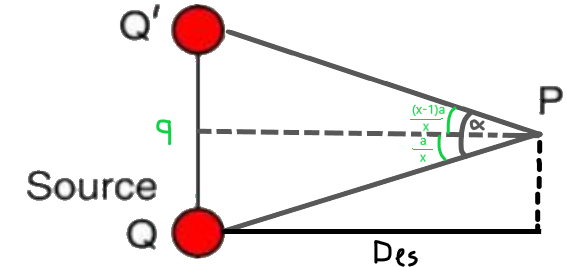
\includegraphics[scale=0.45]{Figures/driehoek.png}
    \caption{Close-up van de desbetreffende driehoek}
    \label{fig:driehoek}
\end{figure}
Er wordt opgemerkt dat $|QQ'| = |Qq|+|qQ'|$. Die twee afstanden zijn makkelijk te vinden uit de tangens. De hoek $\alpha$ wordt gesplitst in twee hoeken (die optellen tot $\alpha$). Zo wordt een rechthoekige driehoek verkregen. De eerste hoek is dan $\frac{\alpha}{x}$. De tweede hoek is gegeven door $\frac{(x-1)\alpha}{x}$. Zo zijn de twee afstanden gegeven door
$$\tan\left(\frac{\alpha}{x}\right)=\frac{|Qq|}{D_{ls}}$$
$$|Qq|=\tan\left(\frac{\alpha}{x}\right)D_{ls}$$
Analoog wordt er gevonden
$$\tan\left(\frac{(x-1)\alpha}{x}\right)=\frac{|qQ'|}{D_{ls}}$$
$$|qQ'|=\tan\left(\frac{(x-1)\alpha}{x}\right)D_{ls}$$
De som is dan gegeven door
$$|QQ'|=D_{ls}\left(\tan\left(\frac{\alpha}{x}\right)+\tan\left(\frac{(x-1)\alpha}{x}\right)\right)$$
Doordat de hoek $\alpha$ klein is kan er Taylor toegepast worden op de tangens, rond 0. Dan wordt er gevonden dat
\begin{align}
    |QQ'| &=D_{ls}\left(\frac{\alpha}{x}+\frac{x\alpha}{x}-\frac{\alpha}{x}\right) \nonumber\\
    &=D_{ls}\alpha
    \label{for:QQ'}
\end{align}
Nu de afstanden $|OQ|, |OQ'|$ en $|QQ'|$ gekend zijn (zie \cref{for:OQ}, \cref{for:OQ'} en \cref{for:QQ'}), kan de lensvergelijking gevonden worden. Het is eenvoudig in te zien dat $|OQ'|=|OQ|+|QQ'|$. Daaruit volgt
\begin{align}
    D_{s}\theta &=D_{s}\beta + D_{ls}\alpha \nonumber\\
    \theta &= \beta + \frac{D_{ls}}{D_{s}}\alpha \nonumber\\
    \beta &= \theta - \frac{D_{ls}}{D_{s}}\alpha
    \label{for: lensvgl}
\end{align}
\cref{for: lensvgl} wordt de lensvergelijking in 1D genoemd.
\onecolumn
\mbox{}
\section{Opbouw afschatten parameters van een sersic}
Voor de afschatting van de parameters van deze appendix werden 7\_500\_000 samples gegenereeerd, waarvan er 10\_500\_000 weggegooid werden.
\label{appendix: opbouw}
\begin{figure}[H]
    \begin{minipage}{0.95\textwidth}
        \centering
        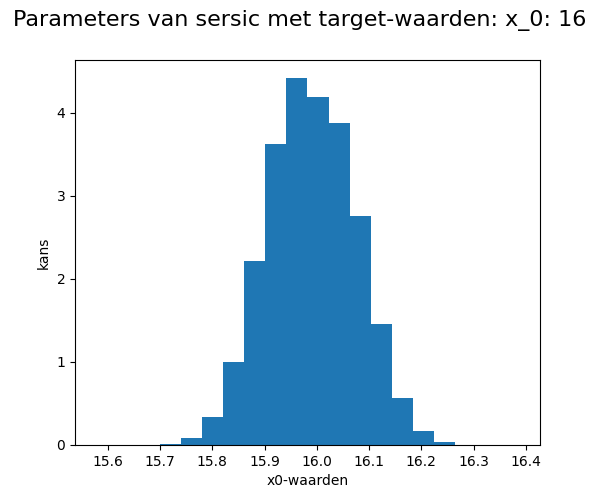
\includegraphics[width=0.3\textwidth]{Figures/1_sersic_verschillende_parameters/sersic_parameters_metropolis_7500000_1500000_10_x0_0.png}
        \subcaption[width=0.3\textwidth]{1 onbekende parameter}
        \centering
        \vspace{1cm}
        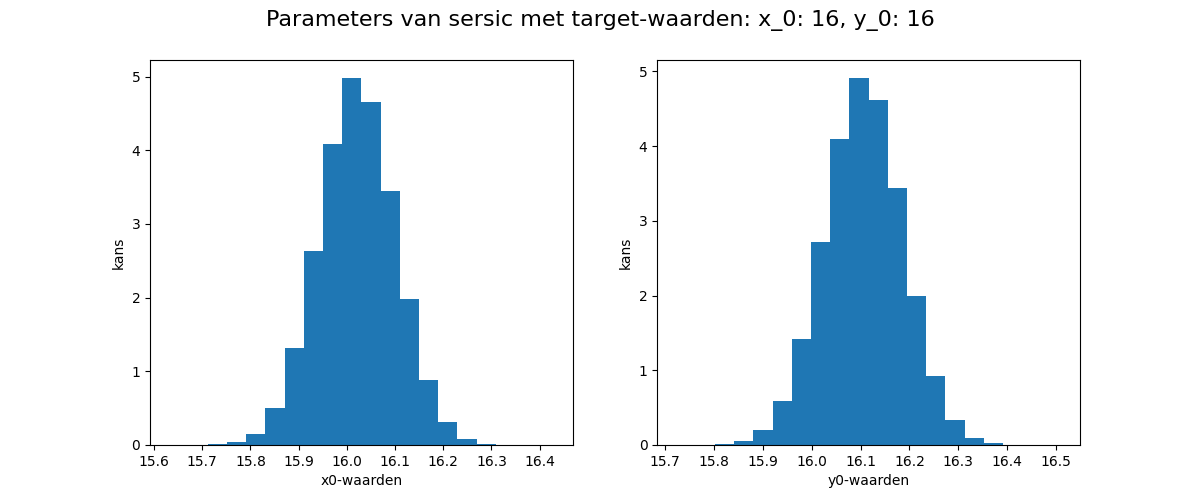
\includegraphics[width=0.60\textwidth]{Figures/1_sersic_verschillende_parameters/sersic_parameters_metropolis_7500000_1500000_10_y0_0.png}
        \subcaption[width=0.6\textwidth]{2 onbekende parameters}    
        \centering
        \vspace{1cm}
        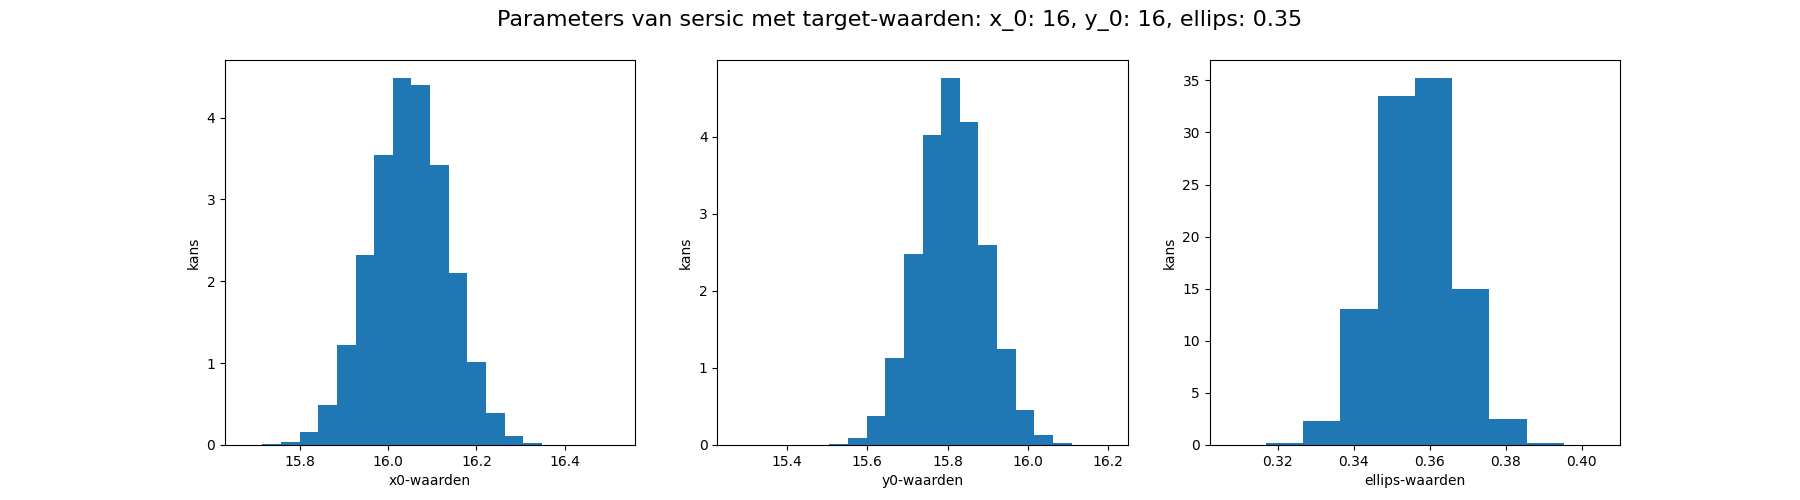
\includegraphics[width=0.93\textwidth]{Figures/1_sersic_verschillende_parameters/sersic_parameters_metropolis_7500000_1500000_10_ellips_0.png}
        \subcaption{3 onbekende parameters}
    \end{minipage}
    \caption{Het proces waarin telkens meer onbekende toegevoegd worden. Er wordt begonnen met één ongekende parameter, en toegewerkt naar drie onbekenden.}
    \label{fig:1 onbekende}
\end{figure}
\begin{figure}
    \begin{minipage}{0.95\textwidth}        
        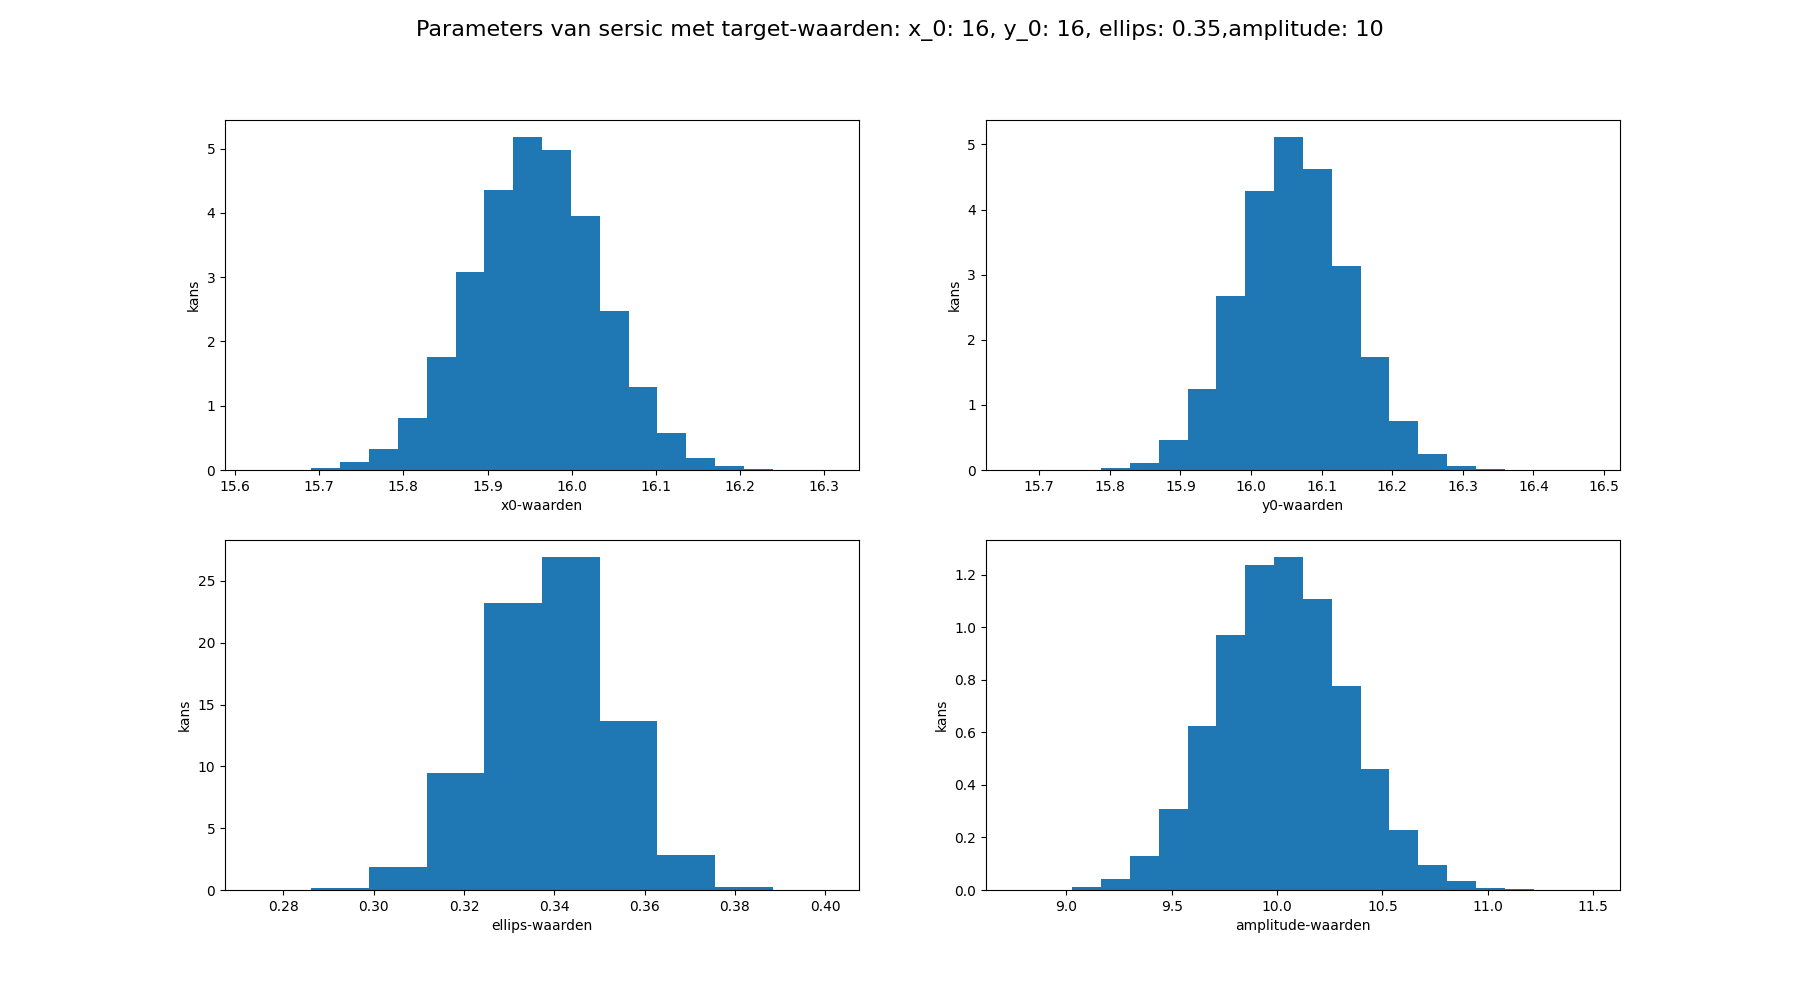
\includegraphics[width=0.93\textwidth]{Figures/1_sersic_verschillende_parameters/sersic_parameters_metropolis_7500000_1500000_10_amplitude_0.png}
        \subcaption{4 onbekende parameters}
        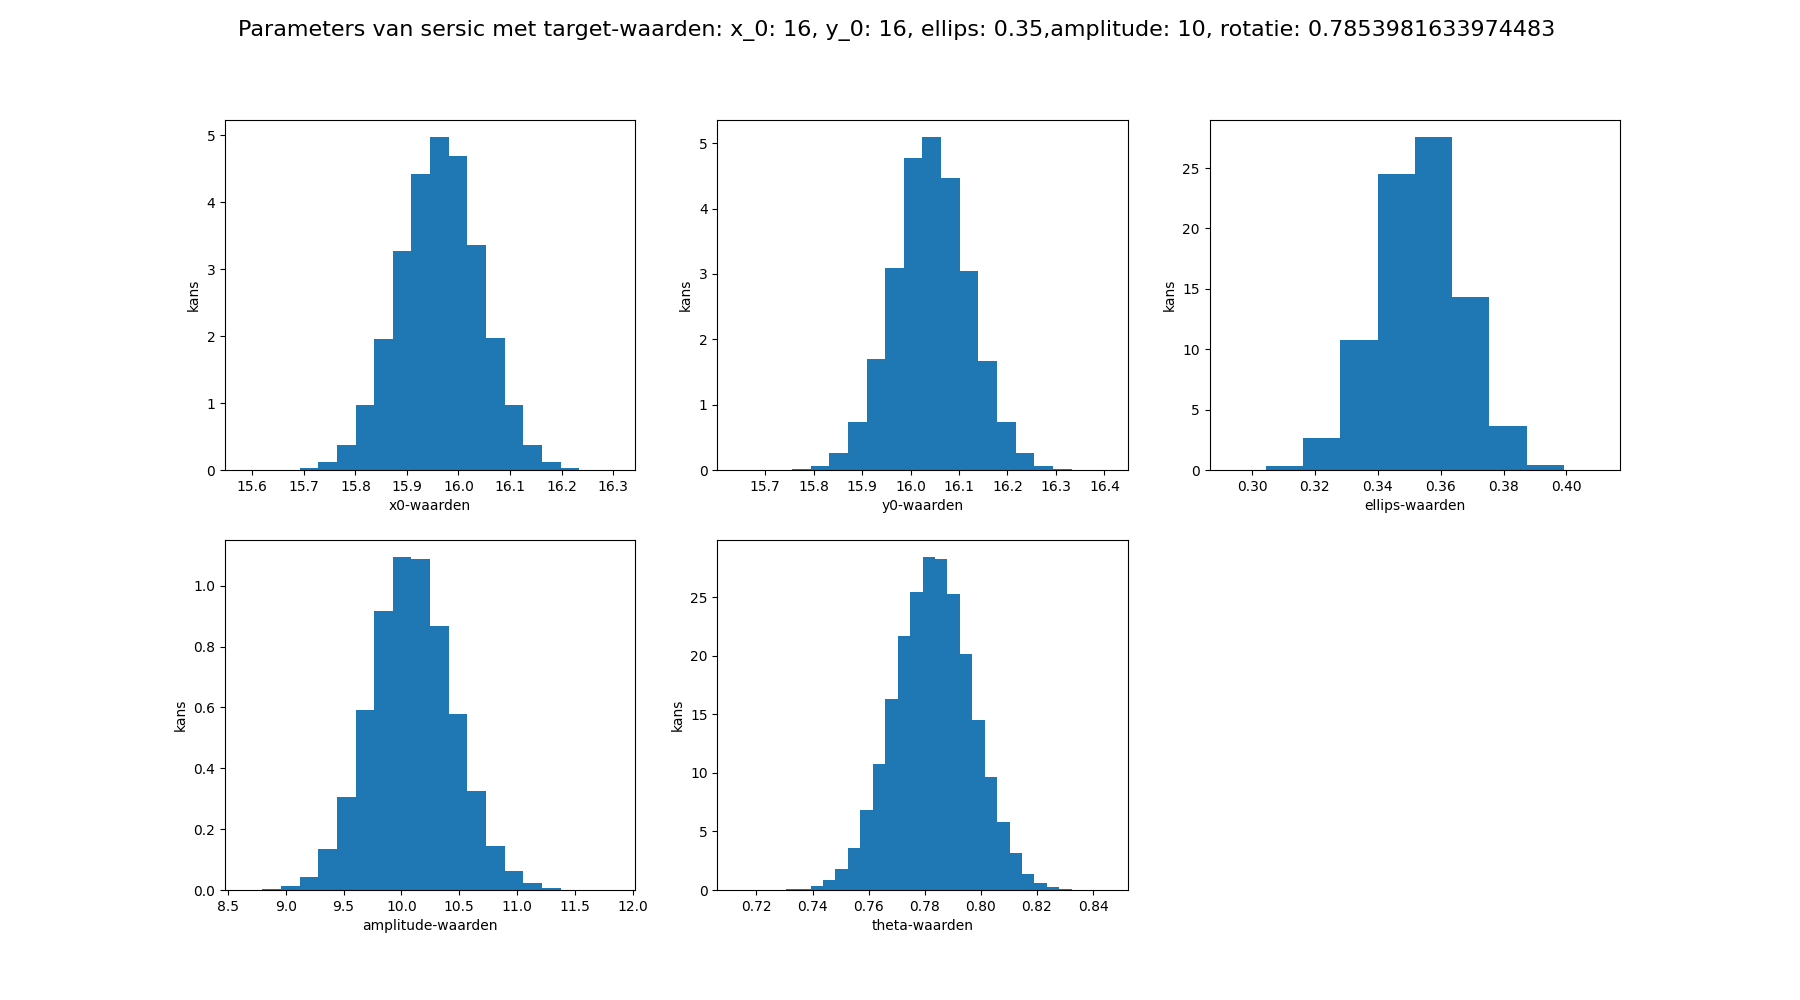
\includegraphics[width=0.93\textwidth]{Figures/1_sersic_verschillende_parameters/sersic_parameters_metropolis_7500000_1500000_10_theta.png}
        \subcaption{5 onbekende parameters}
    \end{minipage}
    \caption{Het proces waarin telkens meer onbekende toegevoegd worden. Er wordt begonnen met vier ongekende parameters, en toegewerkt naar vijf onbekenden.}
    \label{fig:4 onbekenden}
\end{figure}
\begin{figure}
    \centering        
    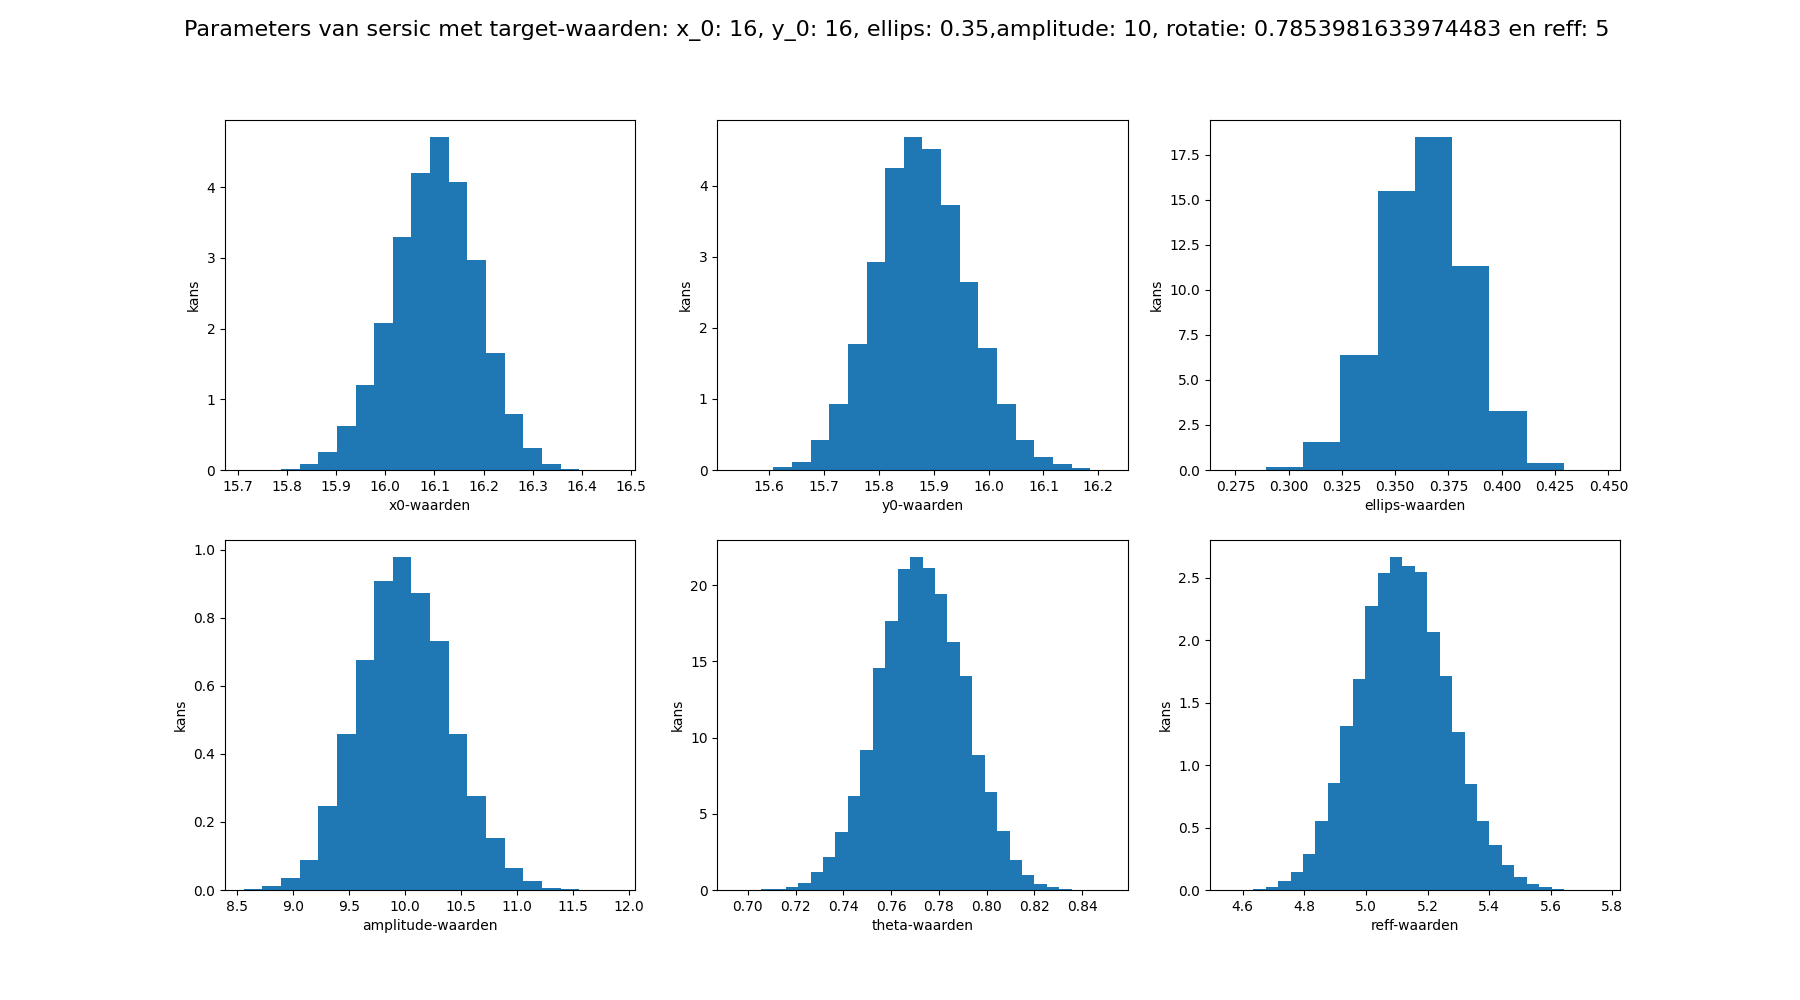
\includegraphics[width=0.93\textwidth]{Figures/1_sersic_verschillende_parameters/sersic_parameters_metropolis_7500000_1500000_10_reff_0.png}
    \caption{Het resultaat van het proces, waarin er zes onbekende parameters afgeschat worden.}
    \label{fig:6 onbekenden}
\end{figure}
\newpage
\twocolumn
% The bibliography is added at the end of the paper in a single column
\newpage
\twocolumn
\printbibliography[title={REFERENCES}]

\end{document}